% Eine der drei folgenden Dokumentenklassen muss gewählt werden.
% Für alle Abgaben außer der finalen Endabgabe darf das 'final'
% Schlüsselwort NICHT gesetzt sein.
% Weitere Hinweise sind im Leitfaden zu finden.

%\documentclass[12pt,titlepage,draft]{book}	% Erstellen der Arbeit und Erstabgabe
%\documentclass[12pt,titlepage]{book}		% Korrigierte Erstabgabe
\documentclass[12pt,titlepage,final]{book}	% Finale digitale und gedruckte Abgabe

%\usepackage[ngerman]{babel} % Deutsche Version

\usepackage[english]{babel} % Englische Version

\usepackage{iflang}




\usepackage{em-thesis} % Erweitert Klasse book
% Hier werden automatisch die folgenden Pakete geladen:
% fontenc, inputenc, graphicx, makeidx, fancyhdr, 
% array, colortbl, xcolor, longtable, xspace

% Hier weitere eigene Pakete einfügen

\usepackage{listings}
\lstdefinelanguage{JavaScript} {
	morekeywords={
		break,const,continue,delete,do,while,export,for,in,function,
		if,else,import,in,instanceOf,label,let,new,return,switch,this,
		throw,try,catch,typeof,var,void,with,yield
	},
	sensitive=false,
	morecomment=[l]{//},
	morecomment=[s]{/*}{*/},
	morestring=[b]",
	morestring=[d]'
}

\usepackage{color}

%New colors defined below
\definecolor{codegreen}{rgb}{0,0.6,0}
\definecolor{codegray}{rgb}{0.5,0.5,0.5}
\definecolor{codepurple}{rgb}{0.58,0,0.82}
\definecolor{backcolour}{rgb}{0.95,0.95,0.92}
\lstset{
	frame=tb,
	framesep=5pt,
	basicstyle=\footnotesize\ttfamily,
	showstringspaces=false,
	keywordstyle=\ttfamily\bfseries\color{blue},
	identifierstyle=\ttfamily,
	stringstyle=\ttfamily\color{codegreen},
	commentstyle=\color{codegray},
	%rulecolor=\color{Gray},
	xleftmargin=5pt,
	xrightmargin=5pt,
	aboveskip=\bigskipamount,
	belowskip=\bigskipamount
}

%\usepackage{amsmath} %Erweiterte Satzmöglichkeiten für Mathematik
%\usepackage{mathpazo} %Palatino-Schrift

% hyperref sollte als letztes Paket geladen werden; dieses ermöglicht Links in PDF
% Hinweis: Die Verwendung von hyperref fuehrt noch zu identifier-Warnungen wg.
%          unterschiedlicher Seitennummerierung.
\usepackage[plainpages=false, pdfpagelabels]{hyperref}

%\usepackage[dvipdfm]{graphicx}
%\usepackage{bmpsize}


%%Informationen fuer die Titelseite
\thesisauthor{Felix Kiechle}
\matrikel{1454042}
\thesistype{Master thesis}
\thesistitle{Design and Development of a Business-Game-Architecture for Round-Based Games:\newline Business Game Description (BGD) and Business Game Engine (BGE)}
%\thesissupervisors{Prof. Dr. Andreas Geyer-Schulz} % Form bei einem Betreuer
\thesissupervisors[M.Sc. Fabian Ball]{Prof. Dr. Andreas Geyer-Schulz} % Form bei zwei Betreuern
%Startdatum ist optional, bei Nichtgebrauch einfach die Zeile löschen oder auskommentieren
%\thesisstartdate{08.\ Januar 2011}
\thesisenddate{11.\ January 2016}

% Beispiele für Trennhilfen, falls Fremdworte oder Spezialausdrücke nicht richtig getrennt werden
% Wichtig! 
% Im german-paket sind zusätzlich folgende Trennhinweise enthalten:
% "- = zusätzliche Trennstelle
% "| = Vermeidung von Ligaturen und mögliche Trennung (bsp: Schaf"|fell)
% "~ = Bindestrich an dem keine Trennung erlaubt ist (bsp: bergauf und "~ab)
% "= = Bindestrich bei dem Worte vor und dahinter getrennt werden dürfen
% "" = Trennstelle ohne Erzeugung eines Trennstrichs (bsp: und/""oder)

% Trennhinweise für Wörter hier beschreiben
\hyphenation{
% Pro-to-koll-in-stan-zen
% Ma-na-ge-ment  Netz-werk-ele-men-ten
% Netz-werk Netz-werk-re-ser-vie-rung
% Netz-werk-adap-ter Fein-ju-stier-ung
% Da-ten-strom-spe-zi-fi-ka-tion Pa-ket-rumpf
% Kon-troll-in-stanz
}

\makeindex
\begin{document}

% 
\ifoptionfinal{}{%
\IfLanguageName{ngerman}{
	\thispagestyle{empty}

%% Beginn Deckblatt
\framebox[\textwidth][l]{
\begin{minipage}{.95\textwidth}
\vspace{2mm}
{\Huge Fassung vom \today} \\

\vspace{\baselineskip}
{\Large \textbf{Achtung:} Dieses Deckblatt ist \textbf{nicht} Bestandteil der gebundenen Fassung dieser Arbeit! Es dient nur zur Versionskontrolle, falls z.B.~vorgezogene Abgaben an den Betreuer stattfinden. Für die finale (digitale) Abgabe kann das Einbinden an der entsprechenden Stelle in der Hauptdatei unterbunden werden. Dazu muss der Status des Dokuments auf 'final' gesetzt werden. Alternativ kann die Seite mit einem passenden Tool aus der PDF-Datei bzw. nach dem Drucken entfernt werden.}
\end{minipage}
}

\vfill

\clearpage


}{
	 \thispagestyle{empty}

%% Beginn Deckblatt
\framebox[\textwidth][l]{
\begin{minipage}{.95\textwidth}
\vspace{2mm}
{\Huge Version dated \today} \\

\vspace{\baselineskip}
{\Large \textbf{Attention:} This cover sheet is \textbf{not} part of the bound version of this work! It is intended for version control, e.g. if early contributions to the tutor take place. For the final (digital) submission the inclusion can be suppressed in the latex main file. Therefore the document status has to be set to final. Alternatively this page can be removed with an appropriate tool from the PDF file, or after printing.
}
\end{minipage}
}

\vfill

\clearpage


}
 \blankpage % Leerseite auf Titelrückseite
}

% Titelseite einbinden
\IfLanguageName{ngerman}{
	%% Titelseite
%% Vorlage $Id: titelseite.tex,v 1.2 2001/01/24 20:13:25 bless Exp bless $
\titlehead{\includegraphics*[width=4cm]{em_includes/kit_logo_de_4c_positiv}} % end titlehead

\begin{titlepage}
%\let\footnotesize\small \let\footnoterule\relax
\begin{center}
\hbox{}
\vfill
{\usebox{\thesistitlesaveone}\par}
\vskip 1cm
\usebox{\thesistypesave} am Lehrstuhl f\"ur Informationsdienste und elektronische M\"arkte\\
\usebox{\thesissupervisoronesave}\\
Institut f\"ur Informationswirtschaft und Marketing\\
Fakult\"at f\"ur Wirtschaftswissenschaften\\
Karlsruher Institut f\"ur Technologie\\[2ex]
von\\[2mm]
\textbf{\usebox{\thesisauthorsaveone}}\\
\vspace*{\baselineskip}
Matrikelnummer \usebox{\thesismatrikelsave}
\vskip 1.5cm
Betreuer: \\[2mm]
\begin{tabular}{l}
\usebox{\thesissupervisoronesave} \\
\usebox{\thesissupervisortwosave} \\
\end{tabular}
\vskip 1.5em
\begin{tabular}{ll}
\ifthenelse{\boolean{startdatumtext}}{Tag der Anmeldung: &}{}
\usebox{\thesisstartdatesave} \\
Tag der Abgabe: & \usebox{\thesisenddatesave} \\
\end{tabular}

\vspace*{3em}
% add versioning information
\ifoptionfinal{}{%
  \ifoptiondraft{%
  \Large\drafttext{Draft}%
  }{%
  \Large\drafttext{Preprint}%
  }
}
\end{center}
\vfill
\end{titlepage}
%% Titelseite Ende


}{
	%% Titelseite
%% Vorlage $Id: titelseite.tex,v 1.2 2001/01/24 20:13:25 bless Exp bless $
\titlehead{\includegraphics*[width=4cm]{em_includes/kit_logo_en_4c_positiv}} % end titlehead

\begin{titlepage}
%\let\footnotesize\small \let\footnoterule\relax
\begin{center}
\hbox{}
\vfill
{\usebox{\thesistitlesaveone}\par}
\vskip 1cm
\usebox{\thesistypesave} at Information Services and Electronic Markets\\
\usebox{\thesissupervisoronesave}\\
Institute of Information Systems and Marketing\\
Department of Economics and Business Engineering\\
Karlsruhe Institute of Technology\\[2ex]
of\\[2mm]
\textbf{\usebox{\thesisauthorsaveone}}\\
\vspace*{\baselineskip}
Registration Number: \usebox{\thesismatrikelsave}
\vskip 1.5cm
Supervisor: \\[2mm]
\begin{tabular}{l}
\usebox{\thesissupervisoronesave} \\
\usebox{\thesissupervisortwosave} \\
\end{tabular}
\vskip 1.5em
\begin{tabular}{ll}
\ifthenelse{\boolean{startdatumtext}}{Date of Registration: &}{}
\usebox{\thesisstartdatesave} \\
Date of Submission: & \usebox{\thesisenddatesave} \\
\end{tabular}

\vspace*{3em}
% add versioning information
\ifoptionfinal{}{%
  \ifoptiondraft{%
  \Large\drafttext{Draft}%
  }{%
  \Large\drafttext{Preprint}%
  }
}
\end{center}
\vfill
\end{titlepage}
%% Titelseite Ende


}
\blankpage  %Leerseite auf Titelrückseite

% Erklaerung einbinden
\IfLanguageName{ngerman}{
\thispagestyle{empty}
\vspace*{36\baselineskip}
\hbox to \textwidth{\hrulefill}
\par
Ich versichere hiermit wahrheitsgem\"a{\ss}, die Arbeit selbst\"andig angefertigt, alle benutzten Hilfsmittel vollst\"andig und genau angegeben und alles kenntlich gemacht zu haben, was aus Arbeiten anderer unver\"andert oder mit Ab\"anderung entnommen wurde.

Ich stimme der Publikation dieser Arbeit auf der Webseite der Abteilung f\"ur Informationsdienste und elektronische M\"arkte des Instituts f\"ur Informationswirtschaft und Marketing am Karlsruher Institut f\"ur Technologie (KIT) zu.

Karlsruhe, den \usebox{\thesisenddatesave}

\clearpage





}{
% Auch im Englischen bleibt Declaration auf Deutsch!
%\thispagestyle{empty}
\vspace*{36\baselineskip}
\hbox to \textwidth{\hrulefill}
\par
\textbf{Declaration of Academic Integrity}\\
I hereby declare that this thesis has been written only by the undersigned and
without any assistance from third parties. Furthermore, I confirm that no sources have
been used in the preparation of this thesis other than those indicated in the thesis itself.

I agree to the publication of this work on the website of the Chair of Information Services and Electronic Markets at the Institute Information Systems and Marketing of the Karlsruhe Institute of Technology (KIT).

Karlsruhe, \usebox{\thesisenddatesave}

\clearpage





 \thispagestyle{empty}
\vspace*{36\baselineskip}
\hbox to \textwidth{\hrulefill}
\par
Ich versichere hiermit wahrheitsgem\"a{\ss}, die Arbeit selbst\"andig angefertigt, alle benutzten Hilfsmittel vollst\"andig und genau angegeben und alles kenntlich gemacht zu haben, was aus Arbeiten anderer unver\"andert oder mit Ab\"anderung entnommen wurde.

Ich stimme der Publikation dieser Arbeit auf der Webseite der Abteilung f\"ur Informationsdienste und elektronische M\"arkte des Instituts f\"ur Informationswirtschaft und Marketing am Karlsruher Institut f\"ur Technologie (KIT) zu.

Karlsruhe, den \usebox{\thesisenddatesave}

\clearpage





}
\blankpage  %Leerseite auf Erklaerungsrückseite

\thispagestyle{empty}
Thanks to Jonas Brügner for discussions and ideas on the architecture design and Fabian Ball and Andreas Sonnenbichler for advice on the definition of the framework for round-based games.

\blankpage

%% Verzeichnisse
\pagenumbering{roman}

\tableofcontents
\blankpage

\listoffigures   % Falls gewuenscht, Kommentarzeichen am Anfang entfernen.
%\blankpage

%\listoftables    % Falls gewuenscht, Kommentarzeichen am Anfang entfernen.
%\blankpage



%% Hauptteil
\pagenumbering{arabic}

%%%%%%%%%%%%%%%%%%%%%%%%%%%%%%%%%%%%%%%%%%%%%%%%%%%%%%%%%%%%%%%%%%%%%%%%%%%%%%%%%%%%%%%%
% Hier beginnt die eigenstaendige Ausarbeitung
%%%%%%%%%%%%%%%%%%%%%%%%%%%%%%%%%%%%%%%%%%%%%%%%%%%%%%%%%%%%%%%%%%%%%%%%%%%%%%%%%%%%%%%%

% Tipp: Anstatt direkt hier LaTeX-Code einzutippen, kann der Inhalt in anderen Dateien
%       abgelegt werden und per \input bzw. \include eingebunden werden.
%       Der Unterschied zwischen \input und \include ist der fehlende Seitenvorschub bei 
%       \input
\chapter{Introduction}
\label{cha:intro}

Simulations are an essential tool to teach pilots, power plant operators, managers and experts in complex decision situations. 
Simulations are used to train regular work processes as well as emergencies:
landing a plane during a storm can be best trained with the help of realistic simulators.

Management simulations, also referred to as business games, gaming simulations, business simulations or serious games, are used to train managers, experts and students to get a better understanding of the effects of decisions in complex systems like markets and supply chains. They are designed to teach management principles, strategies, dynamics and sustainability. 
One of the earliest examples is the Beer Distribution Game (beergame) \cite{JForrester1961,jarmain,beergame}.
It demonstrates the dynamics of a supply chain and illustrates the bullwhip effect.

Many business games are round-based. This means that the game is played for one or several rounds and that the players have to take one or several decisions in each round independently from each other. These decisions, and possibly also the decisions from previous rounds, result in one or several outcomes of a round. The players take their decisions based on the game history and based on their individual strategy. 
For example in the Beergame, each player represents a part of the supply chain and has to decide in each round which amount of beer he is going to order. He takes this decision based on the orders from his client in the supply chain, which arrive with a delay of one or several rounds, and based on his inventory. Storing beer results in inventory costs, unfulfilled orders lead to backlog costs. The players are requested to minimise the costs over the whole supply chain while only having local information about the orders they receive and the costs they produce.

Another example is the Salt Seller business game. Here, players have to set prices for a commodity in a competitive market and experience in each round the effects on market share and profit resulting from their decisions \cite{saltseller}. The Salt Seller simulator aims to convey an understanding for the general dynamics of stable markets \cite[p.90ff.]{sterman}.

The goal of this thesis is to provide an architecture with which any round-based business game can be developed easily and played by multiple users. The amount of coding in a computer simulation to realise just the market models of such games is quite manageable. They can be translated into a few input and output variables together with some state-transition-functions, which define how to calculate the outputs from the current inputs and the game history.

The main effort to allow gameplaying for multiple users in a distributed Internet-based environment with Web-Browsers as front-ends lies elsewhere. If developed individually, every game needs to specify its own mechanisms in order to deal with multiplayer synchronization, data base handling and game visualization, which results in a huge overhead. Simulation development becomes unattractive and expensive and it needs computer science know-how which is not always available in the educational background where such games are conceived and played.

This thesis provides the design and implementation of a gaming engine (BGE) which automates the redundant programming parts related to browser-based multiplayer gameplay, including the visualization and storage of game results. It introduces a description mechanism (BGD) for round-based business games within an online editing environment so that game developers only have to implement their simulation or gaming model while the rest is taken care off by the architecture presented in this work.

The outline of the thesis follows the chronology of the research. A first literature review in the next chapter surveys work on a simulation toolkit for round-based games that has been carried out in Japan. Next, a framework for general n-person round-based games is introduced in chapter 3, providing a clear definition of the class of round-based games. As a main contribution of this thesis, chapter 4 proposes an object-based architecture for round-based games, using a general purpose programming language, followed by a prototype implementation employing the most recent (web)technologies.
\chapter{Related work}
\label{cha:related}

After a short review of business games this chapter surveys the work on a framework for round-based games that has been carried out in Japan.

\section{Business games}
\label{sec:bg}

This section provides a brief overview on business games reviewing history, purpose and ways of classification.

\subsection{History and purpose}
\label{subsec:history}

Greco et al. \cite{greco} describe business games (BGs) as games within a business environment that can lead to one or both of the following results: the training of players in business skills (hard and/or soft skills) or the quantitative and/or qualitative evaluation of the players' performances.

Triggered by the integration of developments in war games, operations research, computer technology and education theory, BGs arrived on the scene in the late 1950s for example with the development of the American Management Association (AMA) decision simulation game \cite{ricciardi}.
In the following years, games such as the Beer Distribution Game \cite{beergame,jarmain,JForrester1961} or the Markstrat Simulation Game \cite{JLarreche1977} were released and remained popular until today \cite{stratx}.
An exhaustive survey about the historical development of the field of business games is presented by Wolfe \cite{wolfe93}.

Today the field of business games is influenced by current technology developments such as natural language processing and advanced graphics processing, new business models like learning on demand and online feedback mechanisms based on artificial intelligence \cite{summers}. 
BGs also serve as experimental environment for training computer players, also referred to as artificial agents or virtual opponents, and for studying deviations of human players from rationality.
Furthermore, BGs are used as incentives to make crowd based online work (crowdsourcing) more attractive and effective \cite{rokicki_competitive_2014}.
They are implemented by global enterprises like Google, Microsoft, American Express, Caterpillar, etc.\ to train their employees and managers \cite{uskov_serious_2014}.

Since their inception, the main purpose of BGs has been to teach. 
Over the years BGs have become very popular in management education. 
Nowadays, almost every MBA program requires students to play one or more management simulations, and BGs are even more commonly applied at the undergraduate level \cite{faria}. 
In addition, role-playing in the business game context can improve soft-skills such as team work, leadership, and practicing concepts and skills used in strategic management, marketing, finance, and project management.

\subsection{Taxonomy}
\label{subsec:tax}

Eilon's early taxonomy \cite{eilon} classifies BGs according to design characteristics (computer/ non-computer, total enterprise/functional, ...) and expected use (management training, selling purpose, research). 

Other taxonomies focus on a specific aspect of a game, such as the web technologies used \cite{web} or the skills that are mediated (product development, project management, logistic skills, risk management) \cite{skill}.

A complete taxonomy of BGs is presented by Greco et al. \cite{greco}. It combines and extends previous work \cite{tax1,tax2,tax3} in this field. 
Greco et al. classify BGs along five dimensions: application environment; elements of the user interface; target groups, goals, and feedback; user relation and model.
Each dimension is described by an enumeration of characteristics and sub-characteristics (see \cite{greco}).
A game can be categorised by a subset of all possible characteristics. 

%\section{Realisation of round-based BGs}
%\label{sec:realisationround}

%\subsection{Stand-alone applications}
%\label{sec:standalone}

\section{Stand-alone applications}
\label{sec:standalone}

An implementation of a business game is called stand-alone application if the game is developed from scratch using its own methods for multiplayer synchronization, data base handling and game visualization.

Numerous (round-based) business games exist as stand-alone applications. For example, Jacobs \cite{sa2} or Ravid and Sheizaf \cite{sa1} use Java applets in order to realise the Beer Distribution Game. 

%\subsection{Frameworks}
%\label{sec:framework}

\section{Frameworks}
\label{sec:framework}

In contrast to a stand-alone application, frameworks support game development and game play for a whole class of games. The goal of this thesis is to build such a framework for the class of round-based games. Previous work on this field has been carried out in Japan for several years.

\subsection{Business Model Description Language (BMDL) and Business Model Development System (BMDS)}
\label{subsec:bmdl}

In 1997 a business simulation course of the Tsukuba University in Japan adopted a new approach allowing their MBA students to develop their own business simulations instead of playing existing conventional business games. The experience of creating their own business models was supposed to convey a better understanding of management skills and of good management decisions. Since only few people had the computer skills and the programming experience needed to implement a whole simulator, a simulation toolkit was developed with the intention to enable easy simulation development for everyone. This toolkit, also referred to as compiler, consists of a business model description language (BMDL) and a business model development system (BMDS) \cite{bmdl3, bmdl2, bmdl1}.

\subsubsection{BMDL}
\label{subsub:bmdl}
%\paragraph{BMDL.}

BMDL is a description language especially invented to create business simulations. It supports all the mechanisms needed for round-based business games. The language consists of a set of 17 keywords (commands) of which the most important ones are presented here. A complete specification of the language can be found in the paper \textit{A compiler for business simulations: Towards business model development by yourselves} \cite{bmdl1}.

\begin{description}
\item[Def.] Game independent settings are  defined using the def-command. Every game must define a game name, the maximal number of players as well as the maximal number of rounds to play. In BMDL, players are also referred to as teams.
\item[Gcon\&scon.] Constants are defined using the gcon- or scon-command. The definition of both commands is \textit{gcon/scon constant-name value}. Gcon introduces a single-valued constant. Scon is an enumeration of constants. Here, the number of values must correspond to the number of rounds so that one value exists for each round. An additional value can exist for the initial state of the constant.
\item[Ivar.] This command defines an input variable. In a round-based game, each player has to take one or several decisions in each round. One input variable corresponds to one decision. In BMDL, the domain of input variables is numeric. It can refer to an interval or a fixed set of values.
\item[Tvar.] This command defines a so-called team variable. Its definition is \textit{tvar variable-name initial-value}. A team variable could be described as a calculated, numeric, player-specific outcome of a round. This outcome is calculated accessing the game history and constants. The game history consists of the players' input decisions of the current and of previous rounds as well as the realisation of team variables of previous rounds including their initial-value. Team variable values of the current round can also be accessed if they have already been calculated.
\item[Tlet.] This command defines how a team variable is calculated in each round. Its definition is \textit{tlet expression} while expression is a piece of code using the syntax and the functions of the C Programming Language. 

The following example shows how the tlet-command works. It assumes a simulation with the input variable \textit{price} and the team variables \textit{sales} and \textit{pr}. The profit ratio $pr$ indicates increasing or decreasing profit in the current round compared to the previous round. In BMDL, this would be translated into $tlet \; pr=(sales*price)/(sales@1*price@1)$. It introduces the relative @-notation in order to access variable values of previous rounds. Tables \ref{tab:bmdl1} and \ref{tab:bmdl2} show an example for the first two rounds and two players supposing the initial state of the game as defined in table \ref{tab:bmdl0}.

\begin{table}[ht]
	\centering
    \begin{tabular}{ l| c c c }
      & price & sales & profit ratio (pr) \\
      \hline
      player/team 1 & 0.50 & 60 & 1\\
      player/team 2 & 0.50 & 60 & 1\\
    \end{tabular}
	\caption{Initial state of the example game}
    \label{tab:bmdl0}
\end{table}

\begin{table}[ht]
	\centering
    \begin{tabular}{ l| c c c }
      & price & sales & profit ratio (pr) \\
      \hline
      player/team 1 & 1.00 & 45 & $\frac{45}{30}=\frac{3}{2}$\\
      player/team 2 & 2.00 & 10 & $\frac{20}{30}=\frac{2}{3}$\\
    \end{tabular}
	\caption{Example game in round 1}
    \label{tab:bmdl1}
\end{table}

\begin{table}[ht]
	\centering
    \begin{tabular}{ c| c c c }
      & price & sales & profit ratio (pr) \\
      \hline
      player/team 1 & 3.00 & 5 & $\frac{15}{45}=\frac{1}{3}$\\
      player/team 2 & 2.00 & 15 & $\frac{30}{20}=\frac{3}{2}$\\
    \end{tabular}
	\caption{Example game in round 2}
    \label{tab:bmdl2}
\end{table}
\end{description}

\subsubsection{BMDS}
\label{subsub:bmds}

%\paragraph{BMDS.}

After a business game has been developed in BMDL it must be translated so that multiple players can play against each other in their browsers. 

The module responsible for this translation is referred to as the BMDL translator \cite{bmdl3, bmdl2, bmdl1} or as Game Generator (GG) system \cite{ybg1}. It is a Perl script that reads the BMDL file and generates Common Gateway Interface (CGI) programs written in C. These so-called business-game-runtime-system-components are then deployed on a standard web server and the game can be played by multiple users in the browser. 

The web server also needs to run a database where variable values as shown in the example above can be stored after player-input or after round-calculation and from which variable values can be retrieved for calculations in later rounds.

\subsection{Yokohama Business Game (YBG)}
\label{subsec:ybg}

The work on BMDL and BMDS was quite successful. Students evaluated it as interesting and recommendable to others and requested to use it in further lessons. Most students rated the complexity of the course as moderate compared to an earlier approach where supplementary programming tasks in C made the understanding of business models too difficult \cite{bmdl3, bmdl2, bmdl1}.

In addition to many game implementations within the simulation course, BMDS was used for a business game simulating the selection of investment projects \cite{bmdsinvest}. Moreover, it was extended so that artificial agents could be employed along with real players \cite{bmdsagent1, bmdsagent2}.  

BMDS was further developed as a system called Yokohama Business Game (YBG). The work on YBG was carried on for several years with a first release of YBG1.0 in 2002 and the final release of YBG2007 in 2007. Many games exist for the YBG platform and it is, or has been used in 70 universities including universities in the US, China and France. A public game server\footnote{http://ybg.ac.jp, retrieved on 20 Oct. 2015} is available in Japanese language \cite{ybg1, ybg2}.

The main improvements of YBG are described in the paper \textit{Facilitating Business Gaming Simulation Modeling} \cite{ybg1}. It introduces a web-based game development environment so that BMDL games can be developed remotely without having to invoke the GG script manually. 

This environment includes different mechanisms to facilitate the game development process. A template structures an empty BMDL file into different sections (constants, inputs, outputs) that every game needs to specify. A conceptual game development framework tries to structure the thinking process which has to be gone through in order to create a business game from the first idea to the complete program. 

Above all, the development environment provides means to detect syntax and logical errors in the BMDL code. The latter can only be detected at runtime, which is why YBG introduces two different simulation mechanisms. In the first approach, the person simulating the game manually enters the inputs of each round for each player and checks if this results in the expected outputs. Since this method can be time consuming given a game with many inputs and players, the second approach makes use of artificial agents which are automatically generating the input values.


\chapter{The game class supported by BGE}
\label{cha:gameClass}
This chapter describes the class of games that can be deployed on the business game architecture proposed in this thesis (BGE). It shows common features among these games and introduces a general framework for $n$-player round-based games.
\section{Common features}
\label{sec:common}
All business games that are designed to run on BGE share the following characteristics of which some are based on the taxonomy of Greco et al. \cite{greco}.
\begin{description}
    \item[Browser-based.] The games run in a web browser and include texts and charts. They are played over a computer network (LAN, Internet).
    \item[Single-/multiplayer.] The games are played by one or more players. Each game defines an interval assigning the minimal and maximal number of players. Most BGs will be designed as multiplayer games where at least two opponents compete against each other. Virtual opponents can be integrated with little effort. This permits a single player to play a multiplayer game against virtual opponents or to simulate the game having virtual opponents compete against each other.
    \item[Round-based.] The games are round-based in contrast to e.g.~a flight simulator where interventions within the simulation are almost continuous. 
    In each round (or period), the players take decisions based on the game history and independent from the other players' decision of this round. Every player must enter his or her decision for the next period within a certain time. 
    The time frame to take a decision is synchronised between all parties which means the players act simultaneously. 
    If one party does not respond within the time frame it is removed from the game. Thus all parties have the same time to reflect and take a decision, assuming a fast interconnection with low latency.
    In contrast to games with alternating rounds like for example chess, where one player decides after the other, decisions in round-based business games are taken simultaneously.
    \item[Indirect user interaction.] Interaction between the players is indirect, since they submit their decisions independently from each other. There are no means of direct interactions, e.g. an integrated communication channel. It is open to the game moderator, respectively the intention of the game session in question, whether communication between players is prohibited or not. There is no direct support for team-building eventhough teams can always be realised by allowing several players to play in front of one computer.
    \item[Player evaluation.] 
    The goals of the games are not absolute (as a fixed score on a scale) but relative to the opponents or to previous sessions of the game. In most BGs the players will be evaluated individually. A collective score evaluating the performance of all players together can be implemented as well. 
    \item[Data collection.] The complete game data is stored for later analysis of the players' behaviour and strategies.
\end{description}

\section{{N}-player round-based games}
\label{sec:round}
This section introduces a general framework for $n$-player round-based games by utilizing
inputs, outputs, fixed parameters, state transition functions, a score function, and a stopping condition.
The framework is then applied to the round-based game \textit{stone-paper-scissors}.

\subsection{A general framework}
\label{subsec:framework}

A $n$-player round-based game is defined through the 7-tuple $(In, P, Out, S_0, \mathcal{F}, score, sc)$. 
The index $t \in  \mathbb{N} (1 \le t \le T)$ represents one round from round 1 to round $T$.
A round is also called turn or period.

\begin{description}
    \item[Inputs.] $In = \begin{pmatrix}
        in_1\\..\\in_l
        \end{pmatrix}$
    is a vector of input variables as e.g. $In = \begin{pmatrix}
        price\\marketing\_exp
        \end{pmatrix}$. An input variable is in turn a vector with an entry for every player $n$. The number of input variables $l$ is assumed to be constant in $t$, which means a game has the same inputs in every round. The domain $D(in_i), i \in \{1,\dots,l\}$ has to be chosen depending on the game, generally, $\mathbb{R}$ can be a good choice.
    
    In each round $t$, $n$ players or virtual opponents submit $l$ input values $in_{ij}^{(t)} \in D(in_i), i\in\{1,\dots,l\},$ $j\in\{1,\dots,n\},t\in\{1,\dots,T\}$ which results in the input matrix $In^{(t)}$ with
    \begin{align}
        In^{(t)} = \begin{pmatrix}
        in_{11}^{(t)}&..&in_{1n}^{(t)}\\..&..&..\\in_{l1}^{(t)}&..&in_{ln}^{(t)}
        \end{pmatrix} \in \begin{pmatrix}
        D(in_1) \times \dots \times D(in_l)
        \end{pmatrix}^n. 
    \end{align}
    One could say that $In^{(t)}$ is the instance of $n$ input variable vectors.
    \item[Parameters.] $P$ is a set of fixed parameters (constants), e.g. a pre-defined number of rounds, a minimal/maximal number of players, a timeout to take a decision or an economic constant. $D(p)$ with $p \in P$ is the domain of a parameter.
    \item[Outputs.] $Out = \begin{pmatrix}
        out_1\\..\\out_k
        \end{pmatrix}$
    is a vector of output variables. As with inputs, the number of outputs $k$ is assumed to be constant in $t$. Output variables resemble input variables. They are a vector with length $n$ and their domain $D(out_i),i\in\{1,\dots,k\}$ is game-dependent.
    
    The outcome of a round or rather the game state in $t$ is described by the output matrix $Out^{(t)}$, which sums up the realisation of the output variables in $t$. It is 
    \begin{align}
        Out^{(t)} = \begin{pmatrix}
        out_{11}^{(t)}&..&out_{1n}^{(t)}\\..&..&..\\out_{k1}^{(t)}&..&out_{kn}^{(t)}
        \end{pmatrix} \in \begin{pmatrix}
        D(out_1) \times \dots \times D(out_k)
        \end{pmatrix}^n. 
        \label{eq:output}
    \end{align}
    \item[Initial game state.] The initial game state $S_0$ defines the state of the game at $t \le 0$ before it has been started. It is fully described by the initial state of every output variable and thus 
    \begin{align}
        S_0 := Out^{(0)}.
        \label{eq:s0}
    \end{align}
    \item[State transition functions.] $\mathcal{F}$ is a set of functions transforming the game state from round $t$ to $t+1$. Hence, these functions are used to calculate the game's outputs of a round $t$ from the parameters and the game history. It is $|\mathcal{F}|=k$ which means there exists exactly one transition function per output variable and  $f_i \in \mathcal{F}, i\in\{1,\dots,k\}$ is used to calculate the output variable $out_i$. Each $f_i$ is defined as
    \begin{align} 
        f_i &\colon D(out) \times D(in) \times D(P) \times playerIDs \to D(out_i),  \label{eq:transition2} 
    \end{align} with $playerIDs := \{1,\dots,n\}$.
    
    A game state is an output in time $t$ so that the output matrix from equation \ref{eq:output} can be written as
    \begin{align}
        Out^{(t+1)} = \begin{pmatrix}
        f_1(Out^{(t)}, In^{(t)}, P, 1)&..&f_1(Out^{(t)}, In^{(t)}, P, n)\\..&..&..\\ f_k(Out^{(t)}, In^{(t)}, P, 1)&..&f_k(Out^{(t)}, In^{(t)}, P, n)
        \end{pmatrix} =: f(Out^{(t)}, In^{(t)}, P).
        \label{eq:state}
    \end{align}
    
    The game history can be accessed as
     \begin{align} 
        f(Out^{(t)}, In^{(t)}, P) = f(f(Out^{(t-1)}, In^{(t-1)}, P), In^{(t)}, P).  \label{eq:hist} 
    \end{align}
    
    \item[Score function.] A player's result or score of a round is calculated with the help of the $score$ function. It is 
    \begin{align} 
        score \colon D(P) \times D(out) \times playerIDs \to \mathbb{R},
        \label{eq:score}
    \end{align} with $playerIDs$ as defined before.
    
    In each round the score function is applied for every player and the results are written to a variable $roundScore^{(t)}$ which is a vector of length $n$ just as an input or output variable. The result over all so-far played periods is defined as
    \begin{align}
        accumulatedScore^{(t)} := \sum\nolimits_{s=1}^t roundScore^{(s)}.
        \label{eq:accumulated}
    \end{align}It is possible to define  a collective score function with \begin{align}
        collectiveScore \colon P \times Out^{(t)} \to \mathbb{R}
        \label{eq:collectivescore}
    \end{align} which assesses the performance of all players together for a period $t$.
    \item[Stopping condition.] $sc$ is a stopping condition. If this condition is met, the game ends. A stopping condition can be e.g. a pre-defined number of rounds.
\end{description}
It is important to mention that in many games the players do not receive complete information about all game describing variables.
Additionally, $P$, $\mathcal{F}$, $score$ and $sc$ can be generalised and defined dependent on $t$ as well, e.g. in the German card game \textit{Skat} $\mathcal{F}$ is defined differently when playing \textit{Null}.
Furthermore, all tuple parts could also be made dependent on the number of players $n$.

\subsection{Applying the framework}
\label{subsec:apply}
This subsection provides an easy example for the application of the framework by applying it to the the round-based game \textit{stone-paper-scissors}.

\paragraph{Initialization.}

Utilizing the framework introduced above, stone-paper-scissors can be described as following:

\begin{itemize}
\item $In=\begin{pmatrix}
       choice
        \end{pmatrix}$. In stone-paper-scissors the players solely have to take one decision in each round and decide between one of three options. Therefore, there is only \textbf{one input variable}. It is called $choice$ with $D(choice) = \{stone, paper, scissors\}$.
\item $P = \{maxrounds, minplayers, maxplayers\}$. The rules of stone-paper- scissors are very simple and there are no game specific \textbf{parameters} as for example economic constants. However, every game needs to agree on the number of rounds to be played, the minimal and maximal number of players who can participate in the game as well as the maximal time to take a decision. Since stone-paper-scissors is a 2-player game consisting of three rounds, it is $minplayers = 2$, $maxplayers = 2$ and $maxrounds = 3$.
\item $Out=\begin{pmatrix}
       roundWinner
        \end{pmatrix}$. The only output in stone-paper-scissors is the information about winner and loser of the round or if the round ended in a draw. That being the case, there is only \textbf{one output variable} which is called \textit{roundWinner}. It has the domain $D(roundWinner) = \{-1,0,1\}$ where -1 stands for defeat, 0 for tie and 1 for victory. The initial state $S_0$ of the game is $Out^{(0)} = \begin{pmatrix}
       0&0
        \end{pmatrix}$.
\item $\mathcal{F}=\{calculateRoundWinner\}$. One output to calculate results in \textbf{one state transition function}. This function calculates the output variable $roundWinner$ for a player $i$ and a round $t$ from the input choices of both players as shown in algorithm \ref{alg:roundWinner}. With $calculateRoundWinner \colon I^{(t)} \times \{1,2\} \to \{-1,0,1\}$, the definition of the function is quite simple; it only needs the current inputs in order to determine the new game state. In more sophisticated games the transition functions are more complex accessing the complete game history and $P$ as shown in equation \ref{eq:transition2}.
\item The \textbf{score function} of stone-paper-scissors is also very simple. The score is 1,-1 or 0 for victory, defeat or tie and thus it just returns the result of the $roundWinner$ output variable of the current round. In other games the score function e.g. combines several outputs and weighs them.
\item The \textbf{stopping condition} checks whether the current round $t$ is greater than the pre-defined number of rounds $maxrounds$. Consequently it is $sc: t > 3$.
\end{itemize}
\begin{algorithm}[h]
	\caption{$\mathtt{}$}
	\label{alg:roundWinner}
	\begin{algorithmic}[1]
	    \Function{calculateRoundWinner}{playerID} 
	    \State $choice1 \gets \text{get \textit{choice} of player one for round \textit{t}} $ \Comment{stone=0, scissors=1, paper=2}
	    \State $choice2 \gets \text{get \textit{choice} of player two for round \textit{t}} $
	    \If{$playerID=1$} 
	        \State $diff \gets choice1 - choice2$ 
	    \ElsIf{$playerID=2$} 
	        \State $diff \gets choice2 - choice1$
	    \EndIf
	    \If{$diff = -1 \text{ or } diff = 2$}
	        \State $result \gets 1$
	    \ElsIf{$diff = 0$}
	        \State $result \gets 0$
	    \Else
	        \State $result \gets -1$
	    \EndIf
	    \State \textbf{return} $result$
	    \EndFunction
	\end{algorithmic}
\end{algorithm}

\paragraph{First round.} 

Assuming player one chooses \textit{stone} and player two chooses \textit{paper}. This results in the input matrix
$In^{(1)} = \begin{pmatrix}
stone&paper
\end{pmatrix} = \begin{pmatrix}
0&2
\end{pmatrix}$.

Applying the state transition function $calculateRoundWinner$ for both players in order to transfer the game state to $t=1$ results in the output matrix $Out^{(1)}=\begin{pmatrix}
-1&1
\end{pmatrix}$. The score function returns the same values which leads to $roundScore^{(1)}=\begin{pmatrix}
-1\\1
\end{pmatrix}$ and \newline $accumulatedScore^{(1)}=\begin{pmatrix}
-1\\1
\end{pmatrix}$.

\paragraph{Second round.} It is assumed that $In^{(2)}=\begin{pmatrix}
scissors&scissors
\end{pmatrix} = \begin{pmatrix}
1&1
\end{pmatrix}$, which means the round ended in a draw. For $t=2$ it is $Out^{(2)}=\begin{pmatrix}
0&0
\end{pmatrix}$ which results in  $roundScore^{(2)}=\begin{pmatrix}
0\\0
\end{pmatrix}$ and $accumulatedScore^{(2)}=\begin{pmatrix}
-1\\1
\end{pmatrix}$.

\paragraph{Last round.} With $In^{(3)}=\begin{pmatrix}
paper&scissors
\end{pmatrix} = \begin{pmatrix}
2&1
\end{pmatrix}$ it is $Out^{(3)}=\begin{pmatrix}
-1&1
\end{pmatrix}$, \newline $roundScore^{(3)}=\begin{pmatrix}
-1\\1
\end{pmatrix}$ and $accumulatedScore^{(3)}=\begin{pmatrix}
-2\\2
\end{pmatrix}$. The game ends because the stopping condition is met. Player two wins the game with a total score of $2 > -2$.
\chapter{Architecture design}
\label{cha:architecture}

This chapter describes the requirements for a business-games architecture and shows how a Business Game Description (BGD) mechanism and a Business Game Engine (BGE) can be designed in order to meet these requirements.

\section{Software requirements}
\label{sec:requirements}

\subsection{Description mechanism}
\label{subsec:req:description}

In order to enable game writers to write their own round-based business games a programming language or game-description mechanism is needed which covers all aspects of round-based games as described in section \ref{sec:round}:
\begin{itemize}
\item The game writer must be able to define \textbf{input variables} as well as the input domain. The latter is needed for the validation of user input. Furthermore, he must be able to decide if the players are asked for a variable or predefined input (empty text field vs. checkbox).
\item \textbf{Parameters} must be supported, including the definition of the domain, so that parameter changes can be validated. This is useful if other users than the original game writer have the privilege to change parameter values or to prevent careless mistakes.
\item The description mechanism must support the declaration of \textbf{output variables} as well as the definition of the output domain and the initial state of the variable. Output variables must be linked with a \textbf{state transition function} in order to specify how the output is calculated. This function must be able to access the set of parameters and the game history as described in equation \ref{eq:transition2}. The outputs of previous rounds and of earlier declared output variables of this round should also be accessible in order to facilitate the implementation of the state transition functions. For the rest of this thesis, the term game history will be used in the broader sense including outputs. 
\item Furthermore it must be possible to define a \textbf{score function} and a \textbf{stopping condition}. The latter can be defined for example in form of a parameter indicating the maximal number of rounds.
\end{itemize}

Apart from supporting the pure description features of round-based games, the description mechanism should
\begin{itemize}
\item define an interface for virtual opponents which enables simulations or game sessions with real players against virtual opponents, 
\item provide a mechanism to define questionnaires between game rounds and/or at the beginning or end of the game,
\item provide means to define how round results, game history and results of the entire game are presented to the players.
\end{itemize}

\subsection{Game development environment}
\label{subsec:req:develop}

If the description mechanism from the last subsection is available, the game writer needs a system or process which allows to
\begin{itemize}
\item write games and transmit the game description to the architecture,
\item validate its syntax and semantics and receive feedback on possible mistakes,
\item save and register the game in the architecture if the syntax and semantics check has passed.
\end{itemize}

\subsection{Simulation environment}
\label{subsec:req:simulation}

After having registered a new game it should be made available for simulation. Here, in contrast to a real game session, the inputs for each round and for each player are provided by the simulation environment. Simulation allows the game developer to test the state transition functions and the correctness of the entire game by verifying if a given input results in the expected output. It can further be used to adjust game parameters. The simulation environment should provide means for debugging in order to locate and understand errors which might occur during game execution.

\subsection{Playing environment}
\label{subsec:req:play}

A game which has been successfully registered and proven to work correctly should be made available as online multiplayer game. The playing environment should meet two main requirements:

\begin{description}
\item[Entrance hall.] This describes a mechanism to join players together who want to play the same game. Players should be informed about their waiting status if the minimal number of players for the game is not yet reached. The game is started after the minimal number of players is reached.

Alternatively the automatic starting behaviour could be changed for a manual start triggered by the game creator. The game creator is the first person who joined the game. He might also be given the possibility to add virtual opponents to the game.
\item[Game engine.] \textit{Game engine} describes a system which enables real time game play of multiple users. It must collect the user input and distribute it to an instance, which
\begin{itemize}
\item calculates the outputs by invoking the state transition functions,
\item distributes and shows the results to the players according to the game description,
\item handles timeout if a player does not provide his input decision within a predefined time frame,
\item saves all game states, parameters, etc. to the database for later analysis.
\end{itemize}
The game engine might also provide a mechanism to render questionnaires and display them to the players if included in the game description.
\end{description}

\subsection{Analysis environment}
\label{subsec:req:analysis}

The analysis environment should a) provide a mechanism to retrieve the collected data of all game sessions of a specific game from the database and deliver it to the user for example as csv-export. It might further b) include various possibilities to filter for specific parts of the game data before exporting it or it might c) provide an online view of selected game data.

\section{Business Game Description (BGD)}
\label{sec:bgd}

As seen in the requirements of section \ref{subsec:req:description}, a mechanism is needed with which game developers can write their own round-based business games. This feature is called Business Game Description (BGD) and there are the following two major ways to approach it:

\begin{description}
\item[New programming language.] One possibility would be to invent a new programming language with its own syntax and keywords which meets all requirements from section \ref{subsec:req:description}. The set of keywords could be kept small compared to a conventional programming language and a language exclusively built in order to describe round-based games would be compact and easy to learn. After having defined this language it would be necessary to build either a compiler or a converter to another programming language. Writing a complete compiler for different architectures seems rather unfeasible in terms of resources. Writing a converter would be the second option, which is for example followed in the work of Tsuda et al.~on BMDL \cite{bmdl1} as introduced in section \ref{subsec:bmdl}. Yet, even a converter still needs a parser which complicates the processing of the language \cite{japanisch} and which is error-prone and time-consuming to build. Moreover, libraries or existing projects which could facilitate the implementation of the system do not exist for a newly created language.
\item[General purpose language.] In the second approach the game itself is written in an object-oriented general purpose programming language. For game developers completely new to programming this might pose an obstacle, although it should be quite easy to adopt existing examples in order to create a new game. The use of an existing programming language maintains a high flexibility since almost everything can be expressed and since a large variety of libraries and projects such as syntax highlighting, syntax checking, code reformatting etc. exist which can be used to facilitate the editing process (sections \ref{subsub:verification} and \ref{sub:module:editor}). It is no longer necessary to write a resource-intensive parser which is the main reason for choosing this second approach in order to create the Business Game Description mechanism.
\end{description}

\subsection{BGD object model}
\label{subsec:bgd:model}

Figure \ref{fig:uml} shows the objects which are used in the Business Game Description mechanism. The Game object is the central element of BGD. It holds all methods that are needed to describe a round-based business game. At game development time, the game writer calls these methods in his game code in order to define and retrieve parameters, inputs, outputs and so on as explained in the following subsections. 

Doing so, the game writer does not need to instantiate the Game object in his code. He just calls the methods as if the Game object had been instantiated before. When some players want to play his game and start it, the game engine creates a new instance of Game. It then loads his code from the database and invokes it which will populate this very instance of Game with the parameters, inputs, outputs, state transition functions etc. which are needed to play his game.

\begin{figure}
	\centering
	\includegraphics[scale=0.565]{figures/gameUml.png}
	\caption{UML diagram of the Business Game Description (BGD) model with chapter references.}
	\label{fig:uml}
\end{figure}

\subsubsection{Parameter object}
\label{subsub:parameters}

A parameter is a constant. The parameter object therefore holds two main attributes, which are the parameter name and the parameter value. The first is of type string, the latter can be string or numeric, depending on the game. In most cases, parameter values will be numeric.

As stated in the requirements of section \ref{subsec:req:description} it should also be possible to specify the parameter domain. This is done using a so-called validation expression. A validation expression is an array of one or several expressions represented by strings. Every time the game code is saved to the database, e.g. after it got created or after some changes took place, the parameter value will be matched against each of these expressions, resulting in an error if one of them fails. For example, if a game developer wants to express that the domain of his parameter $p1$ is defined as $p1 \in \{0,1\}$ the validation expression would be $\begin{pmatrix}
"\ge0"\\"\le1"\\"\%1==0"
\end{pmatrix}$, with \% being the modulo operator. If someone would try to set $p1 = 1.5$ the validation would fail at the third expression because $1.5\%1=0.5\neq0$. The concept of validation expressions will also be used to specify the domain of input and output variables as shown in the next subsection.

At game development time, in order to define a new parameter, the game developer calls the \textit{game.addParameter()} method, specifying name, value and the validationExpression, the latter being an optional parameter. At game play, when his code gets invoked, this will implicitly result in the instantiation of a new parameter object by the game engine which will be added to the parameter collection of the game object. 

As shown in equation \ref{eq:transition2} and \ref{eq:score} the state transition functions as well as the score function need access to the set of parameters. In the game code, this is done with the \textit{game.getPara-} \newline \textit{meter()} method. By specifying the name of the requested parameter this method returns the parameter value.

\subsubsection{Variable object}
\label{subsub:variables}

As seen in section \ref{sec:round}, input and output variables play a fundamental role in round-based business games. In BGD, both are defined by passing a \textit{Variable} object to one of the \textit{game.add...Variable()} methods. The exact definition of these methods and the parameters they take will be explained in the following paragraphs. 

When the game is played, the game engine creates a new Game object and executes the game code. The Variable object, which was passed to the function, will be added to the Game object's array of input or output variables, depending on whether it was an instance of InputVariable or OutputVariable respectively. 

In order to retrieve the value of a variable for a given player and a given round, the game developer can use the \textit{game.get()} function. He will need this for example in the state transition functions in order to fetch values of input and output variables from the game history.

If a state transition function $calcOut2$, which calculates output $out2$, retrieves $out1$ of this round, then $out1$ must be added before $out2$, since the output variables are being calculated in the order in which they are added in the game code.

Finally, each Variable object must specify the \textit{name} attribute and the name of the variables must be unique within one game, since it will be used for example in the \textit{game.get()} function as an identifier. The Variable object may further define the $initialValue$ and $calculationFunction$ attribute as shown below.

\paragraph{Input variable.} An input can be defined calling the \textit{game.addInputVariable()} method. This method takes two parameters of which the first one is obligatory and of type \textit{InputVariable}. Thus, in order to create a new input, the game author first has to instantiate a InputVariable object in his game code. 

As seen in the requirements of section \ref{subsec:req:description} two types of inputs exist, such of variable and such of predefined type. Both must specify the \textit{default} attribute. If a player leaves the game before it has ended or if he exceeds the maximal time to take a decision he will be expelled from the game and the default value will be his input for the remaining rounds. 

A variable input type is represented by the \textit{TextField} object. It must specify the \textit{type} attribute for input validation which can either take the value "number" or the value "string". It may additionally specify a validation expression in order to set out the exact subdomain of textual or numeric input.  

The predefined input type can either be of style \textit{checkbox} or \textit{scrolldown}. Both must define an array of values which represent the different options between which the player can choose. Of course, the default value must be one of these options.

An input object may also define the \textit{calculationFunction} attribute which must be of type \textit{Function} and which represents in the context of input variables the interface to virtual opponents. It is defined in the same manner as state transition functions from equation \ref{eq:transition2}. Instead of calculating an output, this function defines how an input can be automatically generated. It is required if the game should be available for simulation or if virtual opponents should be added to games with real players. This is why it is strongly recommended to implement such a function. In most cases it will be enough to return for example a random number, but it also lays the foundation for sophisticated artificial agents since the game author can access the complete game history and use any kind of programming he likes. The concept of \textit{calculationFunctions} will be explained in more detail in the next paragraph about output variables.

An input variable may further define an initial value. This is mathematically not needed, as seen in equation \ref{eq:s0}, which shows that $S_0$ is fully described by the initial states of the output variables. Nevertheless it has proven practical for some game implementations.

\paragraph{Chart.} As presented at the beginning of the last paragraph, the \textit{game.addInputVariable()} method takes two parameters of which the second is an optional Chart object. If it is specified, the players will see a chart in each round which shows the values of this input variable of every player of the previous rounds. The Chart object describes how this chart should look like. Chart objects are not restricted to input variables but are used as a general concept to visualise the outcome of a variable, using the attributes $caption$, $type$, $unit$, $xInit$ and $xIncrement$. So far, the types \textit{pieChart}, \textit{columnChart} and \textit{lineChart} are supported. Per default, columnChart and lineChart show a value (e.g. price) over all previous rounds while pieChart visualises a proportion (e.g. market share) of the previous round. The caption attribute allows to define a title for the chart. Unit defines the unit of measurement (e.g. \%, euros, etc.) of the variable. The xInit and xIncrement attributes are used in columnChart and lineChart to define the entries of the x-Axis.

\paragraph{Output variable.} With \textit{game.addPlayerVariable()} and \textit{game.addRoundVariable()} two \newline  
methods exist in order to introduce a new output variable in the game code. This may seem strange since the framework for round-based BGs from section \ref{sec:round} knows only one type of output. The difference between both can be explained assuming a business game which implements an output variable \textit{market demand} which changes in each period and which is calculated as a random number. In a given period, the market demand is supposed to be the same for each player. Mathematically, it is not necessary to differentiate such an output from one that is different for every player. In the output matrix from equation \ref{eq:output} this market demand variable would just result in one row with identical numbers for every player. However, in terms of programming it makes sense to distinguish between a \textit{Player(output)Variable} and a \textit{Round(output)Variable} since the latter needs to be calculated and stored only once per round while the first needs to be calculated and stored per round and per player. 

Similar as the value of an input variable, the value of an output variable can be retrieved from the game history with the \textit{game.get()} function. In case of a round-specific OutputVariable the \textit{playerID} parameter is optional and is ignored if specified. In case of a player-specific OutputVariable the \textit{playerID} is obligatory, resulting in an error if not specified. The \textit{game.get()} function takes also the \textit{roundIndex} as a mandatory parameter, specifying the round index for which the output value should be fetched. Supposing a BGD implementation where the first round has $roundIndex = 0$ for the rest of this chapter, any access to a negative roundIndex will return the initial state of the variable which is part of the initial game state $S_0$.

Both output-adding methods introduced at the beginning of this paragraph take two parameters: the first being obligatory and of type OutputVariable, the second being an optional Chart object. As with the inputs, the Chart object is used to visualise outputs. In summary, the OutputVariable object resembles InputVariable. It must define the name and the calculationFunction attribute and it should define an initial value and a validation expression.

The \textit{calculationFunction} attribute links the OutputVariable object to a function. This function represents the algorithm which defines how the output is calculated. It is thus the programmatic counterpart to a state transition function as introduced in equation \ref{eq:transition2}. If the function is linked with a player-specific OutputVariable (or an InputVariable as described in the last paragraph) it must be defined with \textit{playerID} as parameter. If it is linked with a round-specific OutputVariable it must be defined without parameters. It must always return a value which is within the domain of the output (or input) variable which it is supposed to calculate. When the game is played, the game engine calls this function every round in order to calculate the output (or input) value. For a player-specific OutputVariable or an InputVariable it will be called for each player with the playerID of the current player passed as parameter. For a round-specific OutputVariable it will be called once per round without parameters. 

Defining an attribute of type \textit{Function} may seem strange. This is why it should be noted here that the programming language used to implement BGD should for the sake of efficiency support first-class functions and closures. The first means that a function is nothing else than an object which can be for example stored in a variable or passed as parameter to another function. Like this the calculationFunction attribute of a Variable object can be of type Function. A closure means that a function has access to the variables from the context from which it was called. The implementation described in chapter \ref{cha:implementation} provides further details on this topic.

As mentioned before, an OutputVariable object should have the initialValue and \newline 
\mbox{validationExpression} attribute which means it is strongly recommended to include them in every game implementation. A missing initialValue means that the game state $S_0$ is not fully described. Any access to the missing part will result in an error. The validationExpression in output variables is extremely useful in order to validate the correctness of the implementation of the state transition functions. If an error in some function or in the interaction between several functions produces an output value which is not within the correct domain, the error from a failing validation expression can accelerate and facilitate the debugging process.

\subsubsection{Score function}
\label{subsub:score}

The game developer can register a score function by passing it as a parameter to the \newline \textit{game.addScore()} method. The score function should look like a \textit{calculationFunction} of a PlayerVariable as described in the last subsection and follow the definition from equation \ref{eq:score}. Consequently it is a function which takes the playerID as parameter and which returns a score value $\in \mathbb{R}$. Every game should implement a score function, since otherwise it won't have a winner and the players cannot get evaluated individually.

Internally, the concept of the score function uses the same mechanism as variables. The \newline \textit{game.addScore()} call will result in the automatic creation of two OutputVariable objects, one being player-specific and one being round-specific. Both are added at the end of the Game object's array of output variables. Since they are added at the end, when playing the game, all other outputs of all previous rounds including the current one have been calculated before and can be accessed in the \textit{calculationFunction} of the two new objects.

The first of these new OutputVariables is called \textit{roundScore} and its \textit{calculationFunction} is the player-specific score function specified by the game developer. The second is called \textit{accumulatedScore}. Its calculationFunction is automatically generated and defined as introduced in equation \ref{eq:accumulated}. If an optional Chart object was passed as second parameter to the \textit{game.addScore()} method, it will be used to visualise the \textit{accumulatedScore} variable which shows in each round the total score of each player so far reached.

The \textit{game.addCollectiveScore()} method is the second score-related functionality of the Game object. Game developers can use it to register a \textit{collective score} function which evaluates the performance of the players altogether in one period as defined in equation \ref{eq:collectivescore}. For example in the \textit{Beergame}, which was described by John Sterman \cite{beergame}, the players are asked to minimise the collective costs over the whole supply chain (collective score) while only having local information about their own costs (individual score). The concept of collective scores can be used to model such a behaviour. Internally it works in the same way as the individual score, adding two OutputVariables \textit{collectiveRoundScore} and \textit{accumulatedCollectiveScore}.

\subsubsection{Questionnaire object}
\label{subsub:quest}

Questionnaires as formulated in the requirements of section \ref{subsec:req:description} can be included to a game by calling the \textit{game.addQuestionnaire()} method in the game code. It takes as first parameter the name of the questionnaire, as second parameter a Questionnaire object and as last parameter a position array.

A Questionnaire object has a name and a position which are implicitly set by the \newline
$addQuestionnaire()$ method. It further holds an array of \textit{Questions}, of which each defines a question name, a question text and an answer. The answer attribute can be either of type string or of type array of strings. If it is of type string it can take the values "string" or "number", indicating a question with variable input which may be textual or numeric. An answer of type array of strings represents a question with predefined answers; each element in the array becomes one of the options between which the player can choose in order to answer the question.

The last parameter, the position array, must be an array of numbers $\in \mathbb{N} \bigcup \{0\}$ defining the point in time where the questionnaire will be shown. This means that the same questionnaire can occur once or several times at different rounds of the game. Each entry in the array stands for a round before which the questionnaire will turn up. A number bigger than the maximal number of rounds of the game means that the questionnaire will appear at the end while 0 indicates that it will appear before the first round of the game.

\subsubsection{Utility and Mathematics object}
\label{subsub:util}

Both utility and mathematics objects provide access to functions which are supposed to facilitate the game development and are not directly supported by the general purpose programming language in which BGD is implemented. So far, one utility and four mathematical functions are exemplarily specified. Future game implementations may bring up the need for further functionality.

\paragraph{Utility.} With \textit{game.util.getWeekNumber()} the game developer can get the calendar week of a date by passing the corresponding date object to this function. This is useful for game implementations where one period consists of one calendar week and their numbering e.g. in a chart should start with the current week.

\paragraph{Mathematics.} There are two mathematical functions \textit{random()} and \textit{randomInt()} which are intended to help with random numbers since those are often needed for implementations of artificial agents. Both take a numeric minimum $min$ and maximum $max$ value as parameter and return a random value $rv$ with $rv \in [min, max)$, where $rv \in \mathbb{R}$ for the first function and $rv \in \mathbb{Z}$ for the second function respectively.

The mathematics functions \textit{proportionalDistribution()} and \textit{inverseDistribution()} are inspired from the BMDL \textit{prop} and \textit{pinv} commands \cite{bmdl1} and are useful for many game implementations. Assuming a game where two players have to decide upon a price $p_1$ and $p_2$ in each period for a product they want to sell. If the market volume is 100 tons ($distrVal$) and $p_1=75$\euro \space ($distrByVal_1$) and $p_2=25$\euro \space ($distrByVal_2$) a proportional distribution of this market would mean that player one can sell 75 tons at 75\euro \space and player two can sell 25 tons at 25\euro. However, the more realistic distribution in this example would be a (proportional) inverse distribution, where player one with the high price can only sell 25 tons and player two with the low price can sell 75 tons.

For player $i$ with $i\in\{1,\dots, n\}$ the proportional distribution is
\begin{align}
    propDistr_i=\frac{distrVal}{\sum_{i=1}^n distrByVal_i}*distrByVal_i,
\end{align}
while the inverse distribution is defined as
\begin{align}
    invDistr_i=\frac{distrVal}{\sum_{i=1}^n propDistr_i^{-1}}*propDistr_i^{-1}.
\end{align}

This reflects the three obligatory parameters of both distribution functions. The first parameter is the \textit{playerID}. The second parameter is called \textit{distributionValue}. It may either be a number or the name of a round-specific output variable. In the example above the distributionValue was 100 (tons). Supposed that the market volume is stored in the round-specific output variable with the name of $marketVol$, this name can just be passed as second parameter to one of the distribution functions. The game engine will then retrieve the value of $marketVol$ for the current round to calculate and set it as distributionValue. Passing the name of a player-specific output variable or of an input variable (which is also player-specific) will result in an error.

The third parameter is called \textit{distributeByVariableName}. This must be the name of a player-specific output variable or the name of an input variable by which the distributionValue should be proportionally or inversely distributed, as e.g. $price$ in the example above. 

The fourth parameter \textit{optionalRoundIndex} is optional. It is an array of (two) numeric entries $\in \mathbb{Z}$. OptionalRoundIndex[0] $\le t,t\in\{1,\dots, T\}$ specifies the round index for the distributionValue, if it refers to a variable. Using the example above it could be e.g.~expressed to always use the market volume of the previous round instead of the current round as distribution value by setting optionalRoundIndex[0] = currentroundIndex-1. \mbox{OptionalRoundIndex[1]} $\le t$
is used as round index for the distributeByVariable. If one or both values are not specified or if the whole parameter is missing, the current round will be used for calculation.

\paragraph{Others.} Last but not least the two functions \textit{game.getCurrentRound()} and \newline \textit{game.getNumberOfPlayers()} should be mentioned for their importance, even though they do not belong to the Mathematics or Utility objects but directly to the Game object. The first returns the index of the current round the game is in at the moment, where the round index for the first round starts at zero. This feature is needed in virtually every state transition function in order to retrieve an in/output of the current round, the previous round, and so on. The second function returns the number of players $playerCount$ that are actually playing the game (at runtime). This is also an important functionality in many implementations since the developer at development time does not know yet how many players are going to play but only provides the minimal and maximal number of players. It can be used to retrieve variable values from the game history for \textit{all} players, using a loop from 0 to $playerCount-1$ and assuming a BGD implementation where $playerIDs =\{ 0,1,\dots, n-1\}$. It is used for example in the collectiveScore function of the Beergame where the costs over all players need to be summed up. 

\subsection{BGD development}
\label{subsec:bgd:develop}

The requirements of section \ref{subsec:req:develop} specify a development mechanism which should allow developers to write, verify and transmit their game code and to register it in the system. Two major approaches to realise this behaviour can be distinguished:

\begin{description}
\item[Manual verification.] The game developer writes his BGD-code in a text editor of his choice and transmits it via email or via an upload mechanism to a central human control instance. This instance performs a manual or semi-automatic check for malicious code and for mistakes. Syntax errors or minor semantic errors can be corrected by the control instance. If the code then works correctly it can be registered in the architecture. If it contains more severe errors the game developer is provided with feedback and asked to review his code.

Since BGD uses a general purpose programming language for game implementation, security concerns must be taken into account, because executing untrusted game code could harm the system. A manual code check would minimise this risk, at least if carried out with proper care. On the other hand it is a rather inflexible, time consuming and expensive solution, because it needs an experienced reviewer who is constantly occupied by game verification. It is unattractive for the game developer as well who wants to have immediate feedback on his implementation and does not want to wait for the reviewing-process.

\item[Automatic verification.] Automatic verification means the installation of a system which automatises all steps previously undertaken by a manual reviewer. This implies that the game developer can upload his code as a file or write it within the system and have it then automatically checked for syntax and semantic errors as well as for malicious code. If the code is free of such errors and can be trusted, it is saved and registered in the system, otherwise the developer is provided with feedback. This approach is preferred since it makes the entire system more attractive and thus more likely to be used for active game development of round-based business games.
\end{description}

\subsubsection{Automatic game verification}
\label{subsub:verification}

The automatic verification system of the BGD development environment must provide feedback on possible errors. It can be differentiated whether the error is related to the syntax or to the semantics of the game code.

\paragraph{Syntax.} The syntax of BGD is defined by the programming language that is used for its implementation. A typical syntax error would be for example a missing bracket. Open source parsers exist for all major programming languages providing feedback if the parsing was successful or if and where problems were detected. All further checks beyond the syntax of the code should only take place after the syntax check has succeeded.

\paragraph{Semantics.} A semantically correct game implementation provides all the mechanisms and objects that are needed to describe a round-based business game as seen in section \ref{subsec:framework} and \ref{subsec:bgd:model}. A semantic test can for example check if all necessary state transition functions are specified but it cannot prove the correctness of their implementation. This can be done only at runtime, for example in a simulation.

With \textit{error}, \textit{warning} and \textit{success} three different alert levels can be distinguished. An error signifies a missing or incorrect implementation of a feature that would always result in failure at runtime. If a semantic error is detected, feedback should be provided and the code should not be tested further or registered in the system. Checks should ensure that

\begin{itemize}
\item all default parameters ($maxrounds$, $minplayers$, $maxplayers$, $timeout$) are specified,
\item all parameter values match against their validation expressions, if provided,
\item each variable has a name and that this name is unique among all variables,
\item at least one input variable is defined,
\item each input variable defines a semantically correct InputType object, which means that all obligatory attributes are set and the default value matches the domain,
\item each output variable specifies a calculation function, 
\item each questionnaire has a unique name, a numeric position array and an array of valid Question objects with at least one entry.
\end{itemize}

Warning or success means that the game can be further tested or registered in the system. A warning signifies a missing feature that might result in failure at runtime. Feedback should be provided and it should be tested that
\begin{itemize}
\item each input variable provides a calculation function because this is for example needed for simulation,
\item each output variable provides an initial value because otherwise the game might fail at runtime if the initial game state is accessed, 
\item each output variable defines a validation expression in order to detect errors in state transition functions and facilitate their debugging, 
\item the game provides a score function.
\end{itemize}

\subsubsection{Security considerations}
\label{subsub:security}

In a client-server architecture the central security-related question is whether the potentially harmful game code gets executed on the server or on the client.

\paragraph{Server-side.} If untrusted code is executed on the server, strong security measures must be taken. The following list shows possible measures with their advantages and disadvantages. All measures can also be used in combination.
\begin{itemize}
\item The code can be searched with the help of regular expressions in order to forbid access to global variables or to critical functionality such as access to the file-system etc. This approach is quite weak and provides only little security since regular expressions are error-prone, need a lot of testing and it is very hard to cover every loophole the attacker might take.
\item When the code or parts of it get executed, a new worker process can be started, executing the piece of code in question. A new process is automatically separated from the process(es) of the server, which means it cannot access the same space of memory. If possible, this process should be started with limited privileges. The ability to do so depends on the technology that is used on the server as well as the platform it runs on. 

In general, this measure requires that the complete inter-process communication between the system and the worker process must be established over a pipe. This implies that all communication objects must be serializable, complicating the implementation of such a system. Depending on the technology used, functionality might exist which facilitates inter-process communication. 

It furthermore results in the creation of many processes since each execution of for example a state transition function means running untrusted code which has to be secured in a new process. Depending on the number of games that currently run on the server and the number of variables and players of each game this measure produces a lot of overhead and can have a significant impact on the server's performance.
\item In order to reduce this overhead one could try to start only one worker process responsible for every execution of untrusted code. In addition to the necessity of inter-process-communication this approach is very hard to synchronise.
\end{itemize}

\paragraph{Client-side.} In the case of BGD, speaking of a client means the browser of the player(s) since all games are supposed to be browser-based. Consequently, security concerns need not be considered when running untrusted code on the client-side since this is done everyday on the internet and taken care off by the browser's sandbox.

\section{Business Game Engine (BGE)}
\label{sec:bge}

The term \textit{Business Game Engine} (BGE) is used for the architecture as a whole. Business Game Description (BGD) as well as all required environments from section \ref{sec:requirements} are thus part of BGE. 

Architecturally, BGE is a client-server environment with a database. One of its modules is the \textit{startpage}, which is comparable to the index.html file or the home page of a website. It should contain a list with the names of all available business games on this instance of BGE and provides access to all environments, namely the development, simulation, playing and analysis environment. The development, simulation and playing environment are further discussed in the following sections.

\subsection{Development environment}
\label{subsec:bge:d&a}

For game development, BGE features the automatic verification development mechanism from section \ref{subsec:bgd:develop}. It consists of the modules \textit{Online editor} and \textit{Feedback screen} and accesses the database. A full implementation provides at least the functionality \textit{create}, \textit{edit} and \textit{delete}.

\begin{description}
\item[Create.] Linked from the startpage the editor module is loaded. The game developer can input his BGD code here. The feedback screen module informs of possible syntax and semantic errors and might inform if parts of the code are considered to be malicious. If all tests have passed, the game code can be allowed to be written to the database, together with an unique game name, a password and optionally additional information about the developer, game content and so on. The password is used to grant access to the privileged operations edit and delete.
\item[Edit.] Linked from the start page in combination with the choice of a specific game from the game list, the game code of this game is loaded into the editor module if the user is privileged to do so. He can then edit and save the game code under the same conditions as described in the \textit{create} functionality. Parameter changes for instance are performed in this way.

In its easiest implementation, the edit functionality just updates the game code in the database. In order to log which version of a game was played in a specific game session, the current game code should be saved together with every game session. Other realisations might forbid editing an existing game which has already been played or implement a code history. The first implies creating a new game for every new version of a game with existing game data, which reduces flexibility. The latter is more expensive to implement since concurrent edits of different clients must by synchronised.
\item[Delete.] This functionality deletes a game from the database if the correct password is provided.
\end{description}

The development environment might also implement a \textit{show code} functionality which shows the code in read-only mode without asking for a password.

\subsection{Simulation and playing environment}
\label{subsec:bge:simplay}

Similar to the edit or delete functionality from above, the simulation and playing environment is linked from the startpage after the user has chosen one specific game he wants to simulate or play.

The Game object introduced in the UML diagram in figure \ref{fig:uml} holds an array of Round and Player objects that were not discussed so far. This is the case, because they cannot be addressed by the game developer at development time but become important at runtime, when simulating or playing the game.

\subsubsection{Player}
\label{subsub:player}

The Player object describes a player using a name, nickname and email address. This selection is only a proposition. In an BGE implementation where only registered users are allowed to play it might be enough to use the playerID since all other information is already available in the database. In an open BGE implementation other player-describing attributes might be added. 

When a player $p1$ wants to play a game called $easyBG$, BGE creates a Player object $p1\_obj$ that describes him and checks among all currently existing Game objects for a game with the name of $easyBG$ that has the \textit{isOpen} attribute set to $true$. If such an object is found, the player joins it, which means $p1\_obj$ is added to the Game object's array of players. If such an object is not found, either because all games of this type have already been started ($isOpen=false$) or because no such game exists at the moment, a new Game object is instantiated. Its name is $easyBG\_obj$, it is open, $p1\_obj$ is the first object in its array of players and it is now waiting for other players to join.

The functionality described above is part of the \textit{entrance hall} module of BGE. Depending on its implementation, the game is started after the minimum number of players is reached or after the game creator (the first player who joined the game) starts the game. In case of the latter, additional virtual opponents can be added to the game, resulting in the \textit{isBot} attribute of their Player objects to be set to \textit{true}. 

In the easiest implementation of the Player object, as  already mentioned at the end of section \ref{subsub:util}, the playerIDs correspond to the indices of the Game object's player array. This means that $playerIDs = \{0,\dots, n-1\}$. Supposing that $p1\_obj.playerID = 1$ this means that $p1$ was the second player who joined the game and that $game.players[1]$ contains $p1\_obj$.

If a game is simulated but not really played, a random number $rand$ of artificial agent Player objects is created, with $rand \in [minplayers, maxplayers] \in \mathbb{N}$ and the game is started immediately. 

\subsubsection{Round}
\label{subsub:round}

Round objects become important after the game has been started. They are used to fully describe the round of a game. When a new round is started, a new Round object is created and added to the Game object's array of rounds. During and at the end of the round, input and output values are written to this Round object. The BGE module responsible for handling games that have been started is called \textit{game engine}.

The content of a Round object, which means the majority of its attributes as well as their domain, is dependent on the game that is played. Let us assume \textit{easyBG} from the example above has the input \textit{price} and two outputs \textit{marketVolume} and \textit{profit}, the first being round-specific and the latter being player-specific. The domain of all three variables is supposed to be numeric. This will result in Round objects with the three game-dependent attributes \textit{price, marketVolume} and \textit{profit} of which the first and the last are of type array of numbers and the second is of type number. If \textit{easyBG} specifies a score function, two more attributes with the name  \textit{roundScore} and \textit{accumulatedScore} of type array of numbers will be added to its Round objects. 

In other words, each player-specific input or output variable is translated into an attribute with the name of the variable and type array of string or array of number. The length of this array is the number of players that are currently playing the game. The realisation of the input or output variable for player $i$, after the input has been decided upon or the output has been calculated, is stored in this array at index $i$, with $i \in playerIDs = \{0,\dots, n-1\}$. A round-specific output variable is translated in an attribute of type string or number which is used to store the realisation of this output variable.

If a BGE implementation uses $playerIDs \neq \{0,\dots, n-1\}$, an additional mapping function $mf$ with
\begin{align}
mf \colon playerIDs \to \{0,\dots, n-1\}
\end{align}
is needed, in order to retrieve a player-specific variable value or to access the corresponding Player object.

The following example illustrates how Round objects are used in the game engine module. Assuming player $p1$ from the last section is playing \textit{easyBG}, the entrance hall module is implemented so that $playerIDs = \{0,\dots, n-1\}$ and the game is in the third round. $P1$ decides to set up a price of 50\euro \space per ton and the market volume of this period as well as his profit is calculated as 300 tons and 8000\euro. This results in $game.rounds[2].price[1]=50$, $game.rounds[2].marketVolume=300$ and $game.rounds[2].profit[1]=8000$. The command to retrieve \textit{p1's} profit of the previous round in the game code would be \newline $game.get('profit', game.getCurrentRound()-1, 1)$.

\subsubsection{Game and simulation flow}
\label{subsub:flow}

This section summarises all necessary steps that must be taken by the entrance hall and game engine module in order to enable game play or simulation, using \textit{easyBG} as example. \newpage

\paragraph{Entrance hall.} \begin{enumerate}
\item First player $p0$ joins the game. Create $p0\_obj$ and set $name=p0$, $isBot=false$ and $abort=false$. The abort attribute is set true if a player leaves a game before finishing it or if he does not decide within the maximal decision time. Additional information such as nickname, email etc. can be asked for as well.
\item Instantiate new Game object and store it in the variable $easyBG\_obj$. Set $ID$ to an unique value, $name=easyBG$, $isOpen=true$ and $currentRound=0$. Add $p0\_obj$ to the $easyBG\_obj.players$ array.
\item Wait for other players and add their objects when they join.
\item Start the game (the game engine module) when $playerCount \in [minplayers, \newline maxplayers].$ If this is only a simulation, skip the previous steps, instantiate a game object with a valid number of artificial agents and immediately start the game.
\end{enumerate}

\paragraph{Game engine.} 
\begin{enumerate}
\item Load the game code of \textit{easyBG} from the database and invoke it. For example, easyBG holds the round-specific output variable $marketVolume$. In the game code this corresponds with the line $game.addRoundVariable(marketVolume\_obj)$. Running this piece of code will add $marketVolume\_obj$ to $easyBG\_obj$'s array of output variables. Recalling the security considerations in section \ref{subsub:security} it is possible to execute the game code either on the server- or on the client-side. An implementation which chooses the first option should assure that $easyBG\_obj$ is renamed to $game$ for any game code execution. A client-side implementation should not bother since one client only plays one game at a time and $easyBG\_obj$ can be named as $game$ in the first place. In this option, however, it must be assured that the game code and the initial state of $easyBG\_obj$ at the end of the entrance hall module are transmitted to every client participating in the game.
\item Set the initial values of all variables. As seen in section \ref{subsub:variables} output and also input variables may define an initial value which forms the initial game state $S_0$. 
\item Start the first or the next round of the game creating a new Round object. Add this object to $easyBG\_obj$'s array of rounds.
\item Present questionnaire(s) to the players if this is a real game and if questionnaire(s) exists which must be shown before this round.
\item Wait for the input values of the players if this is a real game. If this is only a simulation, calculate the input values calling the $calculationFunction$ of each input variable.
\item Calculate the results of this round by calling the $calculationFunction$ of each output variable after all inputs have been submitted. This includes the execution of the score function(s) as seen in section \ref{subsub:score}. Write these values to the Round object. In case of a client-side execution setting the server must first collect the inputs from each player and redistribute them to each client. 

After the calculation on the client-side it might be considered that each client has to transmit the Round object back to the server for fraud detection since a player could manually alter a variable value in the Browser's Javascript console. If such a fraud is detected, which means if not all Round objects submitted are completely identical, the server might abandon the game or take other measures.

Some games need incomplete information, which means the players have to be prevented in general from using the Javascript console in order to debug into the calculation process and check variable values. Client-side code can be rendered unreadable using code obfuscators\footnote{http://yuiblog.com/blog/2006/03/06/minification-v-obfuscation/ retrieved on 24 Jan. 2016}. A BGE implementation is a big project, even an experienced Javascript developer would need a long time to find the calculation process in such an obfuscated code. Additionally, techniques exist to completely disable the User's Javascript console\footnote{http://www.queness.com/post/16151/disable-javascript-console-in-browsers, retrieved on 24 Jan. 2016}.

\item Present the results of this round to the players displaying for example a chart of all variables for which a Chart object was supplied.
\item If this was the last round of the game: Present the final score to each player and save  $easyBG\_obj$ (now containing the complete game history) to the database. In case of a client-side execution each client must first transmit the final state of its Game object to the server and the server must save one of them.

If this was not the last round of the game: Increment the $currentRound$ attribute of $easyBG\_obj$ and go back to step 3.
\end{enumerate}



\chapter{Implementation}
\label{cha:implementation}

This chapter describes which technologies can be used to implement BGE and how a model realisation of the BGE modules can look like. A prototype is available on \newline \textit{http://games.fkmt.de}. 

Currently implemented BGs on this instance are the \textit{beergame} \cite{beergame}, \textit{SaltSeller} \cite{saltseller}, SaltSeller for many players (with a simplified market model), the example game from the BMDL paper \cite{bmdl1}, the \textit{oligopoly game} as well as \textit{stone-paper-scissors}. The game code of the beergame and of stone-paper-scissors is included in the appendix.
\begin{figure}[t]
	\centering
	\includegraphics[scale=0.58]{figures/architecture.png}
	\caption{BGE architecture overview}
	\label{fig:arch}
\end{figure}

\section{Choice of technology}
\label{sec:imp:technology}

Figure \ref{fig:arch} provides an architecture overview of this implementation of BGE. The following sections describe in detail which technologies are being used and for what reason this is done.

\subsection{BGD object model}
\label{sub:imp:BGD}

The first question to arise is the choice of the object-oriented programming language that is used to implement BGD. Recalling the UML diagram from figure \ref{fig:uml} it is obvious that its most straightforward implementation contains a lot of dynamic types:
\begin{itemize}
\item The type of (function)parameters and attributes or the return type are often decided only at runtime, depending on the game which is currently played. A (game)parameter for instance might be a string or a numerical value and the return type of the \newline $getParameter()$ method is consequently either a string or a number.
\item Some functions accept optional parameters as for example an optional Chart object.
\item Some objects must be extended at runtime. The content of the Round object for example is entirely dependent on the game that is currently played.
\end{itemize}
As conclusion it seems advisable to refrain from using a static programming language such as Java, C or C\# and to prefer a scripting language such as Perl, Python or JavaScript. In addition, all of these three scripting languages natively support first-class functions which facilitates the implementation as seen in section \ref{subsub:variables}.

 The success of a BGE implementation depends on whether the platform can be deployed securely without posing potential risks to the server. The list of security measures from section \ref{subsub:security} in order to run untrusted code on the server is neither complete nor easy to achieve. As a consequence, the second option of running all untrusted code in the browser is preferred. This has also the advantage that the server becomes a mere orchestrator and that the clients take all the load for the calculation of the games' market models. JavaScript being natively supported by all browsers is therefore the favoured programming language for this BGD implementation and taken as assumption for the remaining part of this chapter.
 
\subsection{Client-server-communication: the WebSocket Protocol}
\label{sub:imp:cs}

In a multiplayer BG a great deal of realtime synchronization must take place between the server and the participating players/clients. An implementation with client-side game code execution must support at least the following communication steps:
\begin{itemize}
\item A client must be able to request to play a certain game.
\item The server must join clients together who want to play the same game and inform the players to either wait for other players or to start the game if a sufficient number of players has been reached.
\item The players submit input decisions or questionnaire answers to the server.
\item The server must collect these inputs and redistribute them to the clients for output-calculation after all players have submitted their inputs. 
\item If a player does not answer within the maximal decision time or leaves the game before it has finished the server must disconnect this client, record the abort and use default input values for this player for the rounds to come.
\item The clients must submit their output calculation results after each round or at least at the end of the game so that the server can store the game history to the database.
\end{itemize}

The type of communication channel between client and server over the internet is defined by a communication protocol supported by the browser as well as by the server. Communication protocols are part of the application layer of the OSI model and rely on transport protocols such as TCP or UDP. 

HTTP is a frequently used communication protocol in the internet. Here, any message or data or response from the server must be triggered by a request from the client. The communication is uni-directional since a given instance of HTTP cannot be used to send data in both directions, but only from the client to the server or the other way around.

Previous experiences of implementing a multiplayer BG \cite{saltseller} have shown that using HTTP for communication and synchronization between server and clients leads to a rather complex implementation. The game and the round objects must know different states. A round may for example know the states \textit{running} and \textit{done} depending on whether some or all inputs have been submitted by the players. Depending on the combination of the current game state and round state different actions must be taken (e.g.~calculate outputs if all inputs are submitted) and a certain html page must be rendered or the HTTP request must be redirected to the same or to another location.

Since every communication in HTTP must be initiated by the client, each client must send a HTTP AJAX request in a fixed interval (e.g.~each second) checking the new game and round state, which is called HTTP polling. Assuming there are two players A and B. If A has already submitted its input value but B has not done yet, the last round state A knows is \textit{running}. After B has also submitted its input the round state changes to \textit{done} and A sees with a maximal delay of one second that its own round state and the true round state are different. This triggers a reload of the page and the new state combination leads to some action, in this case maybe the calculation of the outputs and the rendering of a result page.

As a summary, the use of HTTP in \cite{saltseller} led to
\begin{itemize}
\item network overhead for HTTP polling, where a better multiplayer synchronization (with a smaller polling interval) results in bigger overhead,
\item a bad user experience due to page reloads,
\item a highly complex code with many HTTP redirects and different state combinations.
\end{itemize}

A lot would be gained if the server could also initiate the communication and for example inform its clients that all inputs have been submitted. Such a behaviour can be realised for instance using the WebSocket Protocol \cite{websocket} which has been introduced in 2011 and which is now implemented in all major browsers. It establishes a full-duplex (bi-directional) communication channel between server and client through which both can send data at any time.

As a main advantage, the WebSocket Protocol significantly facilitates the implementation of the necessary communication steps. It is used for that reason as communication protocol within the playing environment of BGE. All other environments do not need sophisticated synchronization between server and clients, they only load resources from the server. HTTP was built for that use case and is therefore used in all other environments except the playing environment. The following part of this section describes the specification of the WebSocket Protocol.

In inter-process communication (IPC), sockets are the endpoints of a communication channel on which both processes can send and receive data. Inter-process communication between two processes on different machines can be established over a computer network such as the internet. An internet socket is defined by the unique internet address of the machine (IP address), the delivery slot of this instance of communication (port number) and a the name of the transport protocol used (e.g. TCP or UDP), since different protocols can use the same port \cite{bsd}.

Web browsers do not allow to establish a raw communication channel based on e.g. TCP because this would allow malicious scripts to attack various services on the internet listening on such a connection which are not prepared to deal with harmful input. WebSockets add a layer on top of TCP enabling such a bi-directional communication channel between two processes that are explicitly prepared for it. 

For that reason the protocol specifies an URI-based addressing mechanism\footnote{"ws/wss:" "//" host [ ":" port ] path [ "?" query ]}, for example \textit{wss://server.example.com/secureChat}. Therefore, a WebSocket connection is identified by a scheme component (ws or wss for a TLS secured connection), a host, a port (optional, defaults to 80/443) and a resource (optional, consists of path and/or query). Since several hosts can be hosted one one machine and since it is possible to specify a resource this implies that multiple WebSocket services can share one port and/or one IP address \cite{websocket}. 

In order to establish a WebSocket connection the client and the server must perform the WebSocket handshake. WebSockets use TCP and can be optionally secured with TLS. The client initialises the handshake with a HTTP GET request with Upgrade header. Using HTTP and not another protocol for the handshake allows the WebSocket protocol to coexist with the existing HTTP infrastructure sharing port 80/443 with HTTP clients [Ibid.]. 

In order to establish a WebSocket connection with the chat service mentioned above, a client would open a TLS connection to \textit{sever.example.com} and send a HTTPS GET request for the resource~\textit{\textbackslash secureChat}. Among others this request must specify the Upgrade, Host \textit{(server.example.com)}, Origin \textit{(api.mallory.com)} and Sec-WebSocket-Key Headers. The \textit{Origin} Header field is set by the browser indicating the origin of the script trying to access the service. Typically, a server could only allow trusted scripts e.g. from \textit{example.com} in the example above and reject an unknown script from \textit{mallory.com}. This does not replace authentication or input validation because non-browser clients can also establish the WebSocket connection and can easily fake the Origin header [Ibid.]. 

\textit{Sec-WebSocket-Key} is a base64-encoded 16 byte nonce which the server must concatenate with a predefined GUID. If he accepts the client's connection he must send a HTTP response with status code 101 (Switching Protocols) which includes the \textit{Sec-WebSocket-Accept} Header containing the hashed value. The WebSocket connection cannot be established if this value doesn't correspond with the expected value. With this mechanism the server has to prove that he has received and understood the client's handshake accepting only WebSocket connections. This prevents an attacker to send a message over another protocol as e.g. HTTP that looks like a WebSocket message [Ibid.]. It also prevents from tricking non-WebSocket servers to echo a valid WebSocket handshake response in order to establish an unauthorised connection\footnote{http://www.ietf.org/mail-archive/web/hybi/current/msg06551.html, retrieved on 28 Jan. 2016} \footnote{http://www.ietf.org/mail-archive/web/hybi/current/msg01198.html, retrieved on 28 Jan. 2016}.

After the WebSocket connection has been established both server and client can send and receive data which must be framed as specified by the base framing protocol [Ibid.]. Frames may be fragmented which means that the payload data can be splitted into several frames. This has the advantage that intermediaries who know the protocol and which have seen the handshake can do fragmentation according to network needs. It also implies that both client and server can start to send a message before knowing its size and thus do not have to buffer it completely before sending it. Among others, a frame specifies the content type (text, binary, reserved, control frame or continuation of a fragment), the payload length and an optional masking key. 

Clients must always mask every frame with a new 32 bit random nonce which is unpredictable from within the end application providing the data. Servers must never mask a frame. If one party violates this rules, the connection must be closed. The idea behind is that the client application cannot predict how the data appears on the wire. Otherwise there is a chance that cache poisoning attacks can be leveraged on transparent proxies which are often used for example in enterprise networks to cache content \cite{hack}. In some cases, such intermediaries do not properly implement the HTTP Upgrade mechanism causing the WebSocket handshake to succeed while still interpreting the following traffic as HTTP traffic. If an attacking script is then able to predict how the sent data appears on the wire it can send a WebSocket message to an attacking server which looks like a valid HTTP GET request which is for example fetching a script such as \textit{Google Analytics} with the host \textit{google.com}. The server will then send a response containing a compromised script. For the proxy this looks like a valid response from Google and he now caches the compromised script instead of the real one. All users of the proxy requesting Google Analytics will then receive this compromised script instead of the real Google Analytics.


\subsection{Server-side JavaScript}
\label{sub:imp:server}

WebSocket implementations are available for all server-side technologies such as Java EE, .Net, Python or PHP. However, the event-like character of a WebSocket connection seems to be well suited for JavaScript's event-based, asynchronous execution model. 

\subsubsection{Asynchronous execution model of JavaScript}
\label{sub:sub:async}

In the browser, when performing an I/O operations such as requesting remote content via an AJAX call, or when waiting for an user interaction or setting a timeout, JavaScript does not block the process and does not wait for the operation to complete, but continues to run other code that follows next. As soon as the server delivers the content or the user clicks a button or the timer has run down, the code associated with the operation is executed. Listing \ref{lst:javascript} demonstrates this behaviour for a programme that asynchronously fetches the HTML content of a website using the jQuery library.

\begin{lstlisting}[language=Javascript, caption=JavaScript's asynchronous execution model, label=lst:javascript]
jQuery.get('http://games.fkmt.de', callback); // AJAX call
function callback(data) {
    console.log(data); // Prints the HTML content of the requested website 
}
var pi = calculatePi(1000000); // Calculates Pi with 1M decimal places
console.log('Done. Pi = ' + pi); // Prints "Done. Pi = 3.14..."
\end{lstlisting}
In most programming languages which use a synchronous execution model, a similar programme would wait for the response from the requested website and then print its HTML content on the standard output. After that it would  start calculating Pi and finally print \textit{Done. Pi = 3,14...} Hovewer, the JavaScript programme from listing \ref{lst:javascript} behaves differently. In the first line, the HTTP GET request function gets executed with a callback function passed to it as second parameter. Next, the calculation of Pi is immediately started, without waiting for the network to respond. \textit{Done. Pi = 3,14...} gets printed on the standard output as soon as the result has been calculated. If in the meantime the network has delivered, the callback function is executed and the HTML content is printed. Otherwise the callback function printing HTML will be executed as soon as the network responds.

The JavaScript engine achieves this non-blocking behaviour for I/O and other asynchronous operations using a call stack (also referred to as execution stack or just stack), a message queue and an event loop\footnote{http://2014.jsconf.eu/speakers/philip-roberts-what-the-heck-is-the-event-loop-anyway.html, retrieved on 25 Jan. 2016} \footnote{https://developer.mozilla.org/en-US/docs/Web/JavaScript/EventLoop, retrieved on 20 Dec. 2015}. Messages (events) with an associated callback function get enqueued in response to external events, such as a user clicking a button or a response arriving from a HTTP request. The event loop continuously polls the queue for the next message and puts the associated callback function on the call stack if and only if it finds the stack empty.

Running the file\footnote{In the browser, we cannot just read from a file but would typically embed this program in a <script></script> tag of a html file.} containing the example above, the first function to be put on the call stack is an implicit \textit{eval()} function containing all the code from the file, which is similar to the \textit{main()} function in C or in C-derived languages. Next, the \textit{jQuery.get()} function is put on top of that. It calls the \textit{open()} and \textit{send()} functions from the browser-dependant implementation of the XMLHttpRequest\footnote{https://www.w3.org/TR/XMLHttpRequest/, retrieved on 25 Jan. 2016 } Web API\footnote{https://developer.mozilla.org/en/docs/Web/API, retrieved on 25 Jan. 2016}, which is typically implemented in C(++) as part of the browser's rendering engine and which runs separated from the JavaScript engine in another thread of the browser process. The XMLHttpRequest implementation is from now on in charge for sending the HTTP GET request to \textit{http://games.fkmt.de} and waiting for the response, which results in removing all corresponding function calls from the stack of the JavaScript engine and adding it to the stack of the rendering engine. At an unknown time in future, when the response from the network is available, the rendering engine enqueues the callback associated with this event of the available response in the message queue of the JavaScript engine. If and only if its call stack is then empty, the callback function will be put on the call stack by the event loop, which is continuously waiting for new events to arrive.  

In the meantime, immediately after calling \textit{jQuery.get()}, \textit{calculatePi(1000000)} is put on the stack starting its calculation. After it returns, the result is printed on the standard output (the Browser's console). The call stack is now empty since the end of the file has been reached, which means the implicit \textit{eval()} function can be taken from stack as well. The event loop of the JavaScript engine then continuously polls the message queue for the next event that has been enqueued in the past or that will be enqueued in the future and puts its associated callback on the stack and then pauses polling until the stack is empty again. In the example above, this results in printing the HTML content of the requested website on the standard output.


\subsubsection{JavaScript on the server: Node.js}
\label{sub:sub:node}

JavaScript is omnipresent as scripting language in web browsers, but its deployment on server-side is quite new. Ryan Dahl introduced Node.js in 2009 as a "purely evented, non-blocking infrastructure to script highly concurrent programs"\footnote{https://www.youtube.com/watch?v=ztspvPYybIY, retrieved on 03 Apr. 2016}. Thus, the main idea behind Node.js is to provide the programmer with a server-side environment where all I/O (file system, network, IPC, timers...) can only be done in a non-blocking, asynchronous way. For that, Node.js uses the same concepts as a JavaScript engine, which are an event loop and one single execution stack.

In contrast to for example an Apache web server running a PHP or a Java application, Node.js serves all clients within a single thread. This would not be possible if an I/O operations such as querying the database from one request would block the other requests from being served. This is why all I/O in Node.js is non-blocking. If client A requests something from the server's database, which is in computational terms a very slow operation and takes millions of CPU clock cycles, Node will go on serving requests from other clients and call the callback function associated with A's request as soon as the content from the database is available. 

In the conventional synchronous execution model, each client's request is executed in a new thread since a slow database operation would otherwise block the other clients from being served. Since each new thread consumes a little of the server's memory and the context switching also needs some CPU time, the asynchronous model is well-suited to build scalable web applications which can serve a lot of concurrent connections. The developer need not be experienced with complex (thread-related) tasks such as synchronizing resources since each callback is finished and hence all of its function calls have disappeared from the stack before another one is polled by the event loop. It can thus be used to create efficient applications with comparably little effort. Certainly, CPU-intensive tasks such as the calculation of Pi in listing \ref{lst:javascript} block such a single-threaded setting and must be either avoided or additional child processes or clusters must be spawned \cite{nodedoc}, which might make implementations again more difficult.

\begin{figure}
	\centering
	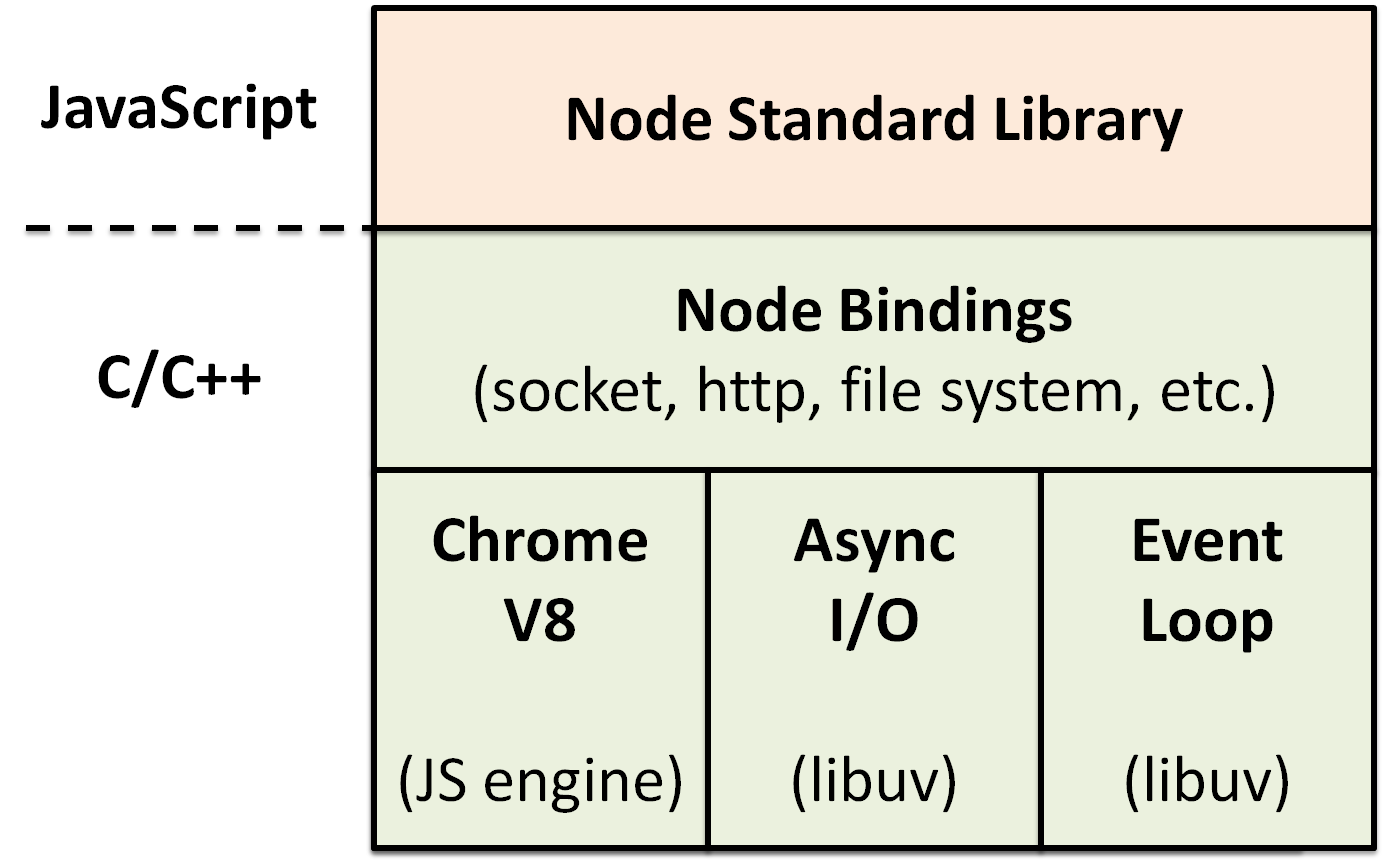
\includegraphics[scale=0.5]{figures/node.png}
	\caption{Node.js architecture overview. Source: stackoverflow.com/questions/36491385}
	\label{fig:node}
\end{figure}
Figure \ref{fig:node} shows an overview of the architecture of Node.js. The API\footnote{https://nodejs.org/api/, retrieved on 04 Apr. 2016} (Standard Library) of Node.js is written in JavaScript and enables the programmer among others to access lower level functionality of the operating system via JavaScript. It is split into different (core) modules providing built-in support for HTTP, TCP, UDP, DNS, TLS, filesystem access, Processes, Buffers, Streams, Events and more. Apart from the core modules, the programmer can import from a large number of other open-source modules via the node package manager (NPM), which has grown the world's largest ecosystem for open-source libraries\footnote{https://www.npmjs.com, retrieved on 04 Apr. 2016}. 

All other parts than Node's API are written in C or in C++. Node.js is built upon Google's JavaScript engine V8. One one hand, V8 is responsible for parsing the user's JavaScript programs and translating it to machine code. On the other hand, V8 provides the Runtime environment, bridging native C++ functions and objects into JavaScript objects. Like this, it is possible to "wrap C++ functions and data structures within JavaScript objects so that they can be manipulated by JavaScript scripts"\footnote{https://developers.google.com/v8/embed\#templates, retrieved on 19 Apr. 2016}. Node.js uses V8 Object and Function Templates to achieve this behaviour. Browsers using V8 apply the same concept in order to expose native implementations of DOM, XMLHttpRequest or other Web APIs to JavaScript and make them available for example as the global \textit{Window} object. 

In Node, most modules of the API have a native C++ counterpart (Node Bindings) providing the actual functionality. For example, the \textit{fs} module in \textit{lib/fs.js} of the API is bound to \textit{src/node\_file.cc} where file system related functionality such as open, read, write, stat and so on can be found. 

However, Node's design goal is to provide purely asynchronous, non-blocking I/O. For example on the network or the file system, asynchronous means that an application expresses interest in a remote resource or a file at one point and uses the data at a different point of time and (memory) space. Non-blocking means that the process was free to do other tasks in the meantime. In UNIX, regular file system I/O is always blocking, while it might be blocking or non blocking in Windows, using a different mechanism\footnote{http://tinyclouds.org/iocp-links.html, retrieved on 08 Apr. 2016}. For asynchronous operations on network sockets, different operating systems provide different system calls\footnote{https://banu.com/blog/2/how-to-use-epoll-a-complete-example-in-c/, retrieved on 08 Apr. 3016}. Node.js and other projects use the C-library \textit{Libuv} in order to realise asynchronous, non-blocking I/O on all major operating systems. It implements an event loop and uses the same callback pattern as JavaScript in order to notify about an incoming event\footnote{http://nikhilm.github.io/uvbook/basics.html, retrieved on 08 Apr. 3016} as well as in order to specify the application logic connected to that certain event. Libuv was created as part of the Node.js project as a replacement for \textit{Libev} when Node was to be ported to Windows. It can be described as a unified interface for asynchronous I/O on all major operating systems. It tries to use the most efficient, non-blocking functionality that each operating system provides for each different type of I/O. When there is no such functionality at all, as for example with file system I/O in UNIX, Libuv uses a thread pool in order to emulate non-blocking behaviour. 

An example: Listing \ref{lst:libuv} shows a simple program that asynchronously reads from a file on the file system, calling Libuv's \textit{uv\_fs\_open()} and \textit{uv\_fs\_read()} functions. Both functions are passed among others a pointer to the event loop, a request object and a callback function. Libuv uses request objects to preserve the context between starting an asynchronous operation and its callback. Thus, the request object is later passed to the callback as parameter. For the rest of this example, the two callbacks are named \textit{on\_open} and \textit{on\_read}. 
\begin{description}
\item[Open.] The \textit{uv\_fs\_open()} call is also passed a path to the file to be opened. Libuv then calls the \textit{open()}\footnote{http://man7.org/linux/man-pages/man2/open.2.html, retrieved on 24 Apr. 2016} facility of the operating system the example program is executed on. If this can be done only in a blocking way, such as on UNIX, Libuv gives this task to a thread pool. Many CPU cycles later, the file system responds with a file descriptor. Libuv then writes this file descriptor to the request object and calls \textit{on\_open}, passing it the request object as parameter. Since the example program is supposed to read from a file, \textit{on\_open } calls \textit{uv\_fs\_read()}, passing it the file descriptor representing the file to read from.
\item[Read.] The \textit{uv\_fs\_read()} call is also passed a buffer. Libuv calls the corresponding \textit{read()} system call\footnote{http://man7.org/linux/man-pages/man2/read.2.html, retrieved on 24 Apr. 2016}, which writes into the buffer. Again, a thread pool is used if necessary. After the data has been read, Libuv writes the number of read bytes to the request object and calls \textit{on\_read} with the request object as parameter.
\end{description}

The event loop and thus a whole Libuv program run as long as there are events to watch out for. The simple example program from listing \ref{lst:libuv} terminates after the open and read have finished. This is described by the two short-lived request objects that preserve the context between start and end of the asynchronous operations. In more elaborate examples, a request represents an asynchronous operation on a long-lived \textit{handle} object. Handles are used to express interests in events on I/O devices, processes or timers. Examples would be a handle on a TCP socket (e.g. for writing a server) or a handle on a pipe (e.g. for streaming from/into a file or for inter-process communication). In this case, the event loop terminates after the socket or the pipe have been closed. 

\begin{lstlisting}[language=C, caption=Libuv example program. \newline Based on https://github.com/nikhilm/uvbook/tree/master/code/uvcat, label=lst:libuv,float,floatplacement=H]
... // Other includes
#include <uv.h> // Include Libuv
static char buffer[1024];
static uv_buf_t uv_buffer;
uv_fs_t open_request; // Create two request objects
uv_fs_t read_request;
void on_read(uv_fs_t *request) {
    fprintf(stdout, "The read data: %s\n", uv_buffer.base);
    fprintf(stdout, "Number of bytes read: %i\n", request->result);
}
void on_open(uv_fs_t *request) {
    uv_buffer = uv_buf_init(buffer, sizeof(buffer));
    uv_fs_read(uv_default_loop(), &read_request,
               *request->result, // Contains the file descriptor
               uv_buffer, ... , on_read);
}
// argv[1] contains the file path
int main(int argc, char **argv) {
    uv_fs_open(uv_default_loop(), &open_request, argv[1], ... , on_open);
    uv_run(uv_default_loop(), UV_RUN_DEFAULT); // Runs the event loop
}
\end{lstlisting}

Recalling figure \ref{fig:node}, how is Libuv to be integrated into the architecture of Node.js? The Node Bindings embed V8 and use it to expose Libuv's functionality to the JavaScript API. Listing \ref{lst:node} translates the C-program from listing \ref{lst:libuv} into a (ES6) JavaScript program. After saving its content to a file named for example \textit{readfile.js}, the program can be executed with the command \textit{node readfile.js /path/to/file}. This will
\begin{itemize}
    \item create a new V8 instance,
    \item create a C++ Process object,
    \item expose this object with V8 as the blueprint for the global \textit{process} object of the Node API\footnote{https://nodejs.org/api/process.html, retrieved on 25 Apr. 2016}, 
    \item additionally add a function called \textit{binding()} to the process object, which is not described in the API but which allows JS code to access the C++ Bindings (this is used in the API core modules), 
    \item make V8 compile and run the startup script in \textit{src/node.js} passing it the process object,
    \item let the startup script install global objects and functions and the module loader in the user space, the latter enabling \textit{require(moduleName)} to load the corresponding (core) module from the API,
    \item read the content of \textit{readfile.js} and run it,
    \item due to \textit{require('fs')} in the source code: load the file system core module and call its \textit{read()} and \textit{open()} functions,
    \item via \textit{process.binding('fs')}, the file system core module calls Read() and Open() from the C++ Bindings,
    \item these functions call Libuv's \textit{uf\_fs\_open()} and \textit{uv\_fs\_read()}, create two request objects and install the callbacks,
    \item start Libuv's event loop calling \textit{uv\_run()} and loop as long for incoming events as there are active handles or requests.
\end{itemize}


\begin{lstlisting}[language=Javascript, caption=Example program in JavaScript using Node.js., label=lst:node]
'use strict';
const fs = require('fs'); // Load the file system core module
fs.open(process.argv[1], 'r', (err, fd)=> { // Arrow functions: ES6
// (err, fd)=> { ... } is here the same as function(err, fd) { ... }
    const buf = Buffer.alloc(1024); // Safe buffer alloc (Node v.5.10.1+)
    fs.read(fd, buf, 0, 1024, null, (err, bytesRead, buffer)=> {
        console.log('The read data: ', buffer.toString('utf8'));
        console.log('Number of bytes read: ', bytesRead);
    });
});
\end{lstlisting}

 \subsubsection{The big picture: Two event loops and WebSockets}
\label{sub:sub:bigpicture}

WebSockets, as stated at the beginning of this chapter, fit perfectly into the asynchronous, event-based execution model of JavaScript and Node.js. Both server and client can send an event, which is nothing more than a string, together with payload data at any time of the connection to the other side. Here, a listener must be defined for that specific event specifying a callback function. Whenever this specific event is sent, the listener is aware of the listened event and executes a callback function with the payload data passed as parameter. 
Table \ref{tab:engine} in the next chapter specifies the concrete events and payload data that are used for the playing environment.

Figure \ref{fig:loops} summarises the main idea of this BGE implementation: Architecture-wide use of the expressive JavaScript programming language and of event-driven, asynchronous programming. WebSockets, needed for the complex synchronisation in the playing environment, fit seamlessly into that concept. 

\begin{figure}[ht]
	\centering
	\includegraphics[scale=0.6]{figures/loops.png}
	\caption{BGE architecture: Two event loops and WebSockets.}
	\label{fig:loops}
\end{figure}

Following this reasoning, Node.js is seen to be an ideal server-side technology for the implementation of BGE. The WebSocket library \textit{Socket.io}\footnote{http://socket.io/, retrieved on 6 Dec. 2015} is very easy to use and drastically simplifies realtime synchronizations between server and clients. The web server realised with the framework \textit{Express}\footnote{http://expressjs.com/, retrieved on 6 Dec. 2015} in combination with the command-line tool \textit{forever}\footnote{https://github.com/foreverjs/forever/, retrieved on 6 Dec. 2015} proved to be sufficient for setting up and maintaining the architecture on a Linux server with very limited physical resources.

Yet the main reason for choosing Node.js was another. Using JavaScript on the server significantly facilitates the development process and maintains a very high flexibility since both client and server speak the same language. In the beginning it was for example considered to execute game code on the server-side. After the security measures from section \ref{subsub:security} turned out to be very hard to realise, the already existing BGE code could be shifted to the client without having to change anything. With Node.js, native JavaScript objects such as the whole Game object serialised as JSON become the data exchange format between server and client. This is -- especially in combination with WebSockets -- a very powerful feature. Sending an object over the internet at any point in the program code and in any direction becomes almost as simple as calling a function.

\subsection{NoSQL Database}

HTTP is a stateless protocol. Due to this fact the database played a central role in the HTTP implementation of the SaltSeller business game \cite{saltseller}. Whenever some change occurred, as for example the calculation of a round's outputs or the game-abort of some player, this change needed to be written to the database. The next HTTP request then fetched the newest state from the database and kept on working with that. Especially when such a system has to serve a lot of games simultaneously, such a frequent database access might become a performance issue.

The WebSocket Protocol is stateful, which means that the connection between server and client is persistent until the client closes or refreshes the tab or redirects or gets redirected to another HTML page. The use case of WebSockets should therefore be well considered since establishing such a connection needs more resources than establishing a HTTP connection. 

For the playing environment of BGE it is indeed worth that effort. Apart from the much simpler implementation, the database becomes a backup tool for later game data analysis rather than a system critical component. In this implementation of BGE, where all calculations are performed by the clients, the game object is initialised on the client side and grows as the game evolves (section \ref{sec:bge}). Only after the game has finished the clients transmit the Game object, now containing the complete game history, to the server, where it gets written to the database. The number of database accesses thus significantly decreases, improving the performance of the architecture.

In consequence, performance indicators such as transactions per second or the maximum number of records that can be stored need not play a major role for the choice of a database technology. Even if a lot of games are played simultaneously the database is unlikely to become the bottleneck of the architecture. 

Much more important are the costs or the effort for saving JavaScript JSON objects. Relational databases are a firmly established technology, using relations (tables) with scalar values (strings, numbers) for data storage. They have been developed for more than 40 years and are widely in use in all industries employing information technology. Their query language SQL is based on the sound mathematical concept of relational algebra and is standardised for almost 20 years. In order to save objects of any object oriented programming language as well as their relationships among each other into a relational database, a mapping mechanism is needed which is referred to as Object Relational Mapping (ORM).

An ORM for the object model of BGD would typically map the Game object to the two relations \textit{game} and \textit{round}. One game consists of many rounds which means each record in the round-table holds the ID of the game to which it belongs (foreign key). The game relation holds everything which stays the same during an entire game, such as information about the players, questionnaires, parameter values and so on. The round relation contains the input and output values of each round of the game as well as questionnaire results. 

Since BGE generically supports round-based games with different data attributes, this mapping cannot be static but must be created dynamically for every individual game. This asks for implementing a model factory which translates a specific game into CREATE TABLE and INSERT INTO statements of a certain relational database management system (RDBMS). Such an implementation is expensive. Depending on the experience of the developer, the number of RDBMSs supported and the test coverage it should take about 10 to 20 full development days. Furthermore, changes applied to an existing game may also affect the data model, for example when introducing a new variable or parameter or questionnaire. If such a change is to be translated into ALTER TABLE statements instead of dropping and recreating the relations, the effort for implementing such an ORM further increases. 

Document-oriented databases, often referred to as NoSQL, non-relational databases or object databases, are a rather young technology. Their main idea is to save documents such as YAML\footnote{http://www.yaml.org/, retrieved on 29 Jan. 2016}, XML or JSON directly without an additional mapping. Since they are quite new, their query languages are not standardised. Each NoSQL database comes with its own query syntax which must be learned by developers or data analysts and which may support more or less features.

MongoDB\footnote{https://www.mongodb.org/, retrieved on 26 Dec. 2015} was one of the first document-oriented databases to arise. It is said to have a rich query language\footnote{https://www.mongodb.com/blog/post/mongodb-vs-sql-day-14-queries, retrieved on 26 Dec. 2015} and a big community\footnote{https://www.mongodb.com/press/mongodb-fastest-growing-community-big-data, retrieved on 26 Dec. 2015} \footnote{55k questions by the end of 2015 on stackoverflow.com. This is quite much for a new technology, SQL in comparison has 300k questions.}. A rich query language means that subsets of the stored data can be retrieved based on various different query criteria. A large community signifies that many online resources such as forums or blog entries exist which allows to familiarise more easily with the new technology. Both points are important if a NoSQL database becomes a potential candidate for BGE.

The ACID properties are another important criterion for the choice of a database technology. ACID stands for \textit{Atomicity}, \textit{Consistency}, \textit{Isolation} and \textit{Durability} and is fully supported by relational databases. Atomicity and Isolation signifies that a transaction (a series of read, write and/or update operations) either completes or fails as a whole and that a concurrency model exists which serialises concurrent data access of different clients. A NoSQL database such as MongoDB does not support this natively. By default, MongoDB only guarantees write operations on a single document to be atomic\footnote{https://docs.mongodb.org/manual/core/read-isolation-consistency-recency/, retrieved on 26 Dec. 2015}. Thus, there are several possibilities how concurrent transactions might run into race conditions, if not prevented by a proper implementation. A series of read and write (depending on what has been read) on a single document might be interrupted and invalidated by another write operation. The same applies for updates on multiple documents, where a document can be seen as the equivalent of a table in a relational database. MongoDB provides functionality and design patterns such as \textit{findAndModify()}, embedded documents or isolation\footnote{https://docs.mongodb.org/manual/core/write-operations-atomicity/, retrieved on 26 Dec. 2015} in order to avoid race conditions. However, unlike with RDBMSs, this must be taken care off by the developer on the application level. In the assessment of a database technology the use-case must be therefore well evaluated. The potential gain from not having to implement ORM might be outweighed by a more complex implementation assuring ACID conformity.

BGE uses the database mainly to save game sessions and to retrieve this data later for game-analysis. A Game object is a single document in terms of NoSQL, writing it to the database is thus an atomic operation. The read operations for data analysis cannot violate ACID since only transactions containing write operations are in danger to do so. The database is also used to save or update game code after creating or editing a business game. The game code is saved together with an unique game name, the authors' names and a game description in a single document. Writing it to the database is thus an atomic operation. This implementation of the development environment from section \ref{subsec:bge:d&a} uses simple updates when a game is edited. In this case the update transaction is also atomic since it is equivalent to a single write operation on a single document. The current game code is saved together with every game session. An example: two clients concurrently edit a game with a time difference of 1 ms and a third client starts a new game session of this game between the two edits. The game version of the first client will be persistent in the database for approximately 1 ms and it will be saved to the game session of the third client. After that the game version of the second client is written to the database.

As a conclusion, the use-case of BGE contains no danger to run into race conditions whatsoever. MongoDB is therefore chosen for this implementation of BGE since it is able to save JavaScript JSON objects natively without having to implement an expensive mapping mechanism. The new query syntax has proven to be expressive and can be easily learned thanks to a big community and a JavaScript-like notation. 

\section{Module realisation}
\label{sec:imp:realisation}

This section describes how the BGE modules $startpage$, \textit{online editor}, \textit{feedback screen}, \textit{entrance hall}, \textit{game engine} as well as the Game analysis environment are implemented on this prototype of BGE.

\subsection{Startpage}
\label{sub:module:startpage}

\begin{figure}
	\centering
	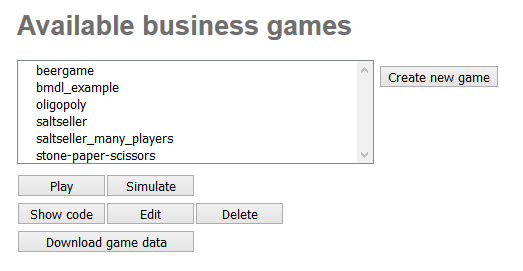
\includegraphics[scale=1]{figures/startpage.png}
	\caption{Startpage module}
	\label{fig:startpage}
\end{figure}

Figure \ref{fig:startpage} shows a realisation of the startpage module with all the business games that are currently available on the BGE implementation on \textit{http://games.fkmt.de}. The create, show, edit and delete buttons link to the development environment as described in section \ref{subsec:bge:d&a}. The other buttons link to the playing, simulation and analysis environment.

\subsection{Online editor and feedback screen}
\label{sub:module:editor}

The online editor module is used in the development, simulation and playing environment. In the development environment it enables to create new business games or to show or to edit the game code of existing games. In the simulation environment the editor displays the results or the errors of the simulation. In the playing environment it is optionally used if turned on in the source code in order to present game results to the players (below the charts).

The feedback screen is used for game validation in the development environment. It shows syntactic or semantic errors when creating or editing a game as described in section \ref{subsub:verification}. Figure \ref{fig:editor} shows the editor and feedback screen module displaying a semantic error.

\begin{figure}
	\centering
	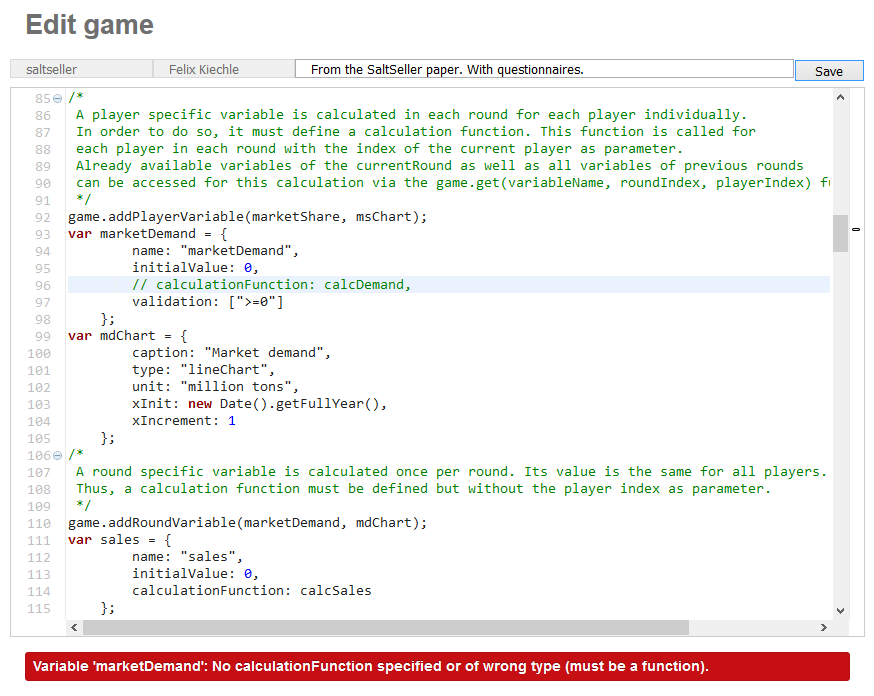
\includegraphics[scale=0.61]{figures/editor.png}
	\caption{Editor and feedback screen module}
	\label{fig:editor}
\end{figure}

The editor is based on the open-source Eclipse project \textit{Orion}\footnote{https://wiki.eclipse.org/Orion, retrieved on 03 Jan. 2016} which aims to create a browser based integrated development environment (IDE). It uses the open-source JavaScript parser \textit{Esprima}\footnote{https://http://esprima.org/, retrieved on 03 Jan. 2016} for the syntax analysis of the game code. Esprima is furthermore used together with the \textit{escodegen} project\footnote{https://github.com/estools/escodegen, retrieved on 03 Jan. 2016} for reformatting the source code after loading it from the database (show or edit). Reformatting is also used for the presentation of simulation results.

\subsection{Entrance hall and game engine}
\label{sub:module:engine}

The entrance hall and the game engine module enable game play and simulation as described in section \ref{subsec:bge:simplay}. The entrance hall is implemented so that the game starts automatically after the minimal number of players is reached and in such a way that $playerIDs = \{0,\dots, n-1\}$.

The game engine implements client-side game code execution. Table \ref{tab:engine} provides an overview of the WebSocket events on server and client and the corresponding actions they trigger. The list is nearly complete. It only misses the \textit{abort} event which is emitted by the client if a player disconnects from the game during game play (closes or refreshes the tab) or does not provide inputs within the maximal decision time. The server then marks the game as aborted in the corresponding Player object and uses default input values or the last input values submitted for the rounds to come in order to allow the other players to continue the game.

This implementation of the game engine module uses Google Charts\footnote{https://developers.google.com/chart/interactive/docs/gallery/piechart, retrieved on 20 Oct. 2015} for rendering Chart objects. Figure \ref{fig:play} shows an example game session of the \textit{SaltSeller} business game after two rounds have been played. Figure \ref{fig:questionnaire} gives an example of a questionnaire.

\begin{table}
	\centering
   \begin{tabular}{ p{7.825cm} | p{7.825cm}  }
      \textbf{Client} & \textbf{Server} \\
    \hline
      - Client connects and is asked to submit nickname \newline
      - \textbf{Emit event "play"}. Data: nickname and gamename &  \\
       ----------------------------------------------------->&  \textbf{On "play"}: \newline 
       - load gamecode from database \newline
       - Create Player object \newline
       - Join existing or create new game \newline
       - \textbf{Emit "wait join"} if minimal player number not yet reached \newline
       - Otherwise: \textbf{emitAll "init"} Data: game code, player objects\\
       \textbf{On "init"}: \newline
       - Instantiate new Game object \newline
       - Run game code \newline
       - Render input fields and questionnaires \newline
       - Wait for input or show questionnaire \newline
       - \textbf{Emit "input"} Data: inputs of all players or save questionnaire results to the Game object when user submits. & <-----------------------------------------------------\\
       ----------------------------------------------------->& \textbf{On "input"}: \newline
       - Save each incoming input data within the object that manages currently running games \newline
       - After all players have submitted input: \textbf{emitAll "calculate"} Data: input data of all players.\\
       \textbf{On "calculate"}: \newline
       - Create round object and write incoming input data to it \newline
       - Calculate round results (output variables) from inputs and write to round object \newline
       - Draw charts \newline
       - If last round: show game results, \textbf{emit "finish"} Data: whole Game object (contains complete game history) \newline
       - Not last round: increment round index, \textbf{emit "result"} Data: calculated round object&\\
       ----------------------------------------------------->&\textbf{On "result"}: \newline
       - NiceToHave: Fraud detection \newline
       - \textbf{Emit "set input"}\\
       &\textbf{On "finish"}: \newline
       - Save Game object to database \\
       \textbf{On "set input"}: \newline
       - Wait for input or show questionnaire \newline
       - \textbf{Emit "input"} Data: inputs of all players or save questionnaire results to the Game object after user submits.&<-----------------------------------------------------\\
      \hline  
    \end{tabular}
	\caption{Socket events on client and server }
    \label{tab:engine}
\end{table}

\begin{figure}
	\centering
	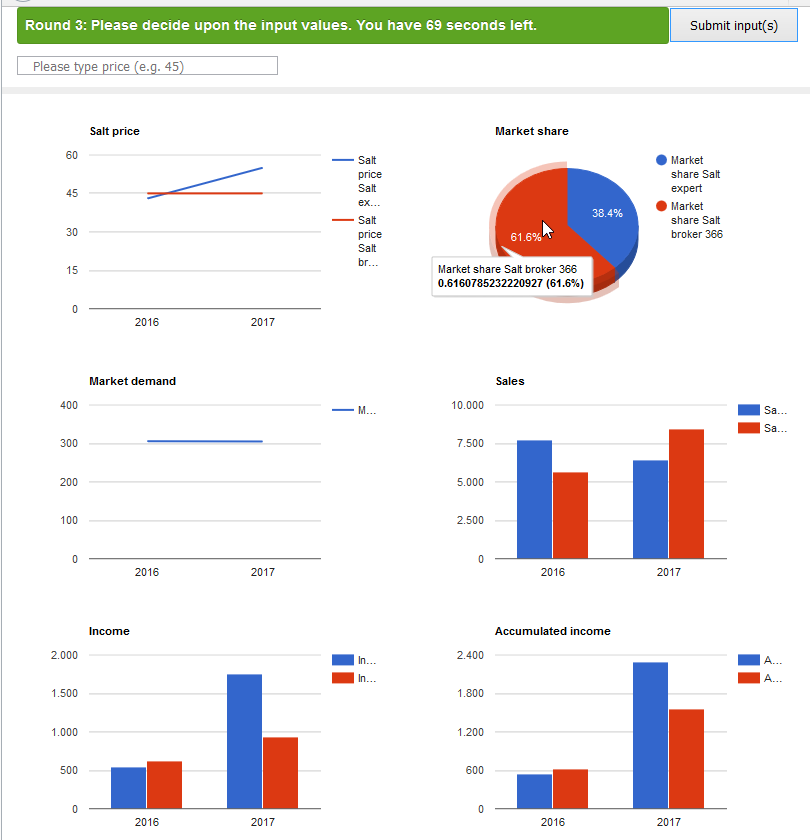
\includegraphics[scale=0.61]{figures/play.png}
	\caption{Screenshot of two players playing the \textit{SaltSeller} business game after two rounds have been played}
	\label{fig:play}
\end{figure}

\begin{figure}
	\centering
	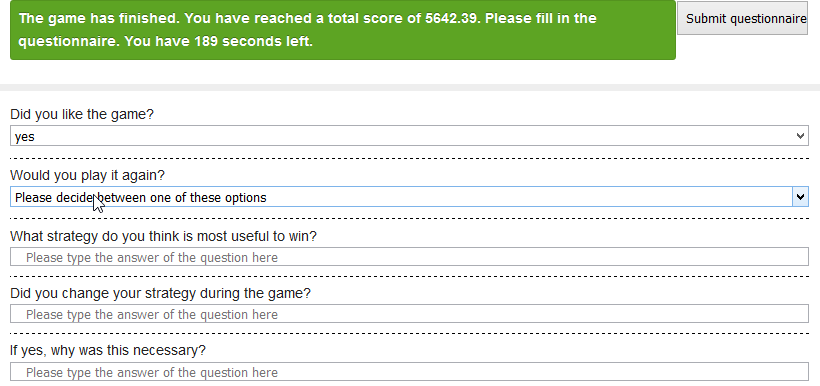
\includegraphics[scale=0.61]{figures/questionnaire.png}
	\caption{Example of a questionnaire which is displayed after the game has finished}
	\label{fig:questionnaire}
\end{figure}

\subsection{Game analysis}
\label{sub:module:analysis}

The entire game data of all game sessions of a specific business game which has been played on this instance of BGE can be downloaded as JSON file using the \textit{Download game data} button on the startpage. JSON is a well readable data exchange format (compared to XML for example) and libraries and utilities exist for all programming languages. 

Future implementations might provide an advanced analysis environment (see the next section) which can reduce the need for data analysts to learn the MongoDB query syntax or to write wrappers around the JSON files.
\newpage
\section{Dependencies}
Table \ref{table:dep} provides a brief overview of the third party libraries used in BGE.
\begin{table}
	\centering
    \begin{tabular}{ | p{5cm} | p{9,65cm} | }
    \hline 
    \textbf{Library} & \textbf{Description} \\
    \hline  
      Node.js \newline https://nodejs.org & Event-driven, non-blocking JavaScript Runtime for the server\\
      \hline  
      MongoDb \newline https://www.mongodb.org  & NoSQL database \\
      \hline 
      mongodb \newline https://www.npmjs.com/\newline package/mongodb 
      & MongoDb driver for Node.js \\
      \hline  
      express.js \newline 
      http://expressjs.com
      & Web server framework for Node.js \\
      \hline 
            socket.io \newline 
      http://socket.io
      & WebSocket implementation for Node.js \\
      \hline 
      esprima \newline 
     http://esprima.org/
      & Open-source JavaScript parser \\
      \hline 
            escodegen \newline 
    https://github.com/\newline estools/escodegen
      & JavaScript code generator (for reformatting) \\
      \hline 
                csurf, bodyparser, cookieparser & Middleware used by express.js for CSRF protection and body/url parsing \\
      \hline 
       jade & Template rendering engine for Node.js (used to insert CSRF tokens) \\
      \hline 
       Google charts  https://dev elopers.google.com/chart/ & JavaScript Chart API \\
      \hline 
    Eclipse orion & Editor for the web-browser \\
      \hline 
          JQuery & JavaScript frontend utilities \\
      \hline
    Foundation \newline http://foundation.zurb.com & CSS framework \\
      \hline
      
    \end{tabular}
    	\caption{BGE dependencies }
    	\label{table:dep}
\end{table}

\section{Installation guide}
\label{sec:imp:installation}

This section provides a brief installation guideline for a Debian based system (e.g. Ubuntu). 

\subsection{Prerequisites}
Install Node.js
\begin{itemize}
    \item \textit{sudo apt-get install npm} --> Installs the node package manager (NPM)
    \item \textit{sudo npm install -g npm} --> Updates NPM to the latest version
    \item \textit{sudo ln -s /usr/bin/nodejs /usr/local/bin/node} --> Syslink to the node environment, maybe only needed on Ubuntu
    \item \textit{sudo npm install -g n} --> install node binary manager \newline (https://www.npmjs.com/package/n)
    \item \textit{n stable} --> install the newest stable version of node
\end{itemize}
Install MongoDB
\begin{itemize}
    \item \textit{sudo apt-get install mongodb}
\end{itemize}

\subsection{BGE installation}

\begin{itemize}
    \item Checkout or copy BGE code to some local folder
    \item Go inside that folder
    \item \textit{npm install} --> Reads package.json in order to locally (inside BGE folder) install all the dependencies needed for BGE (see last section)
\end{itemize}

\subsection{Run it locally}
\begin{itemize}
    \item \textit{node server.js} --> Starts the BGE server, will listen on port 3000
    \item Start a browser, navigate to \textit{localhost:3000}
\end{itemize}
\subsection{Deployment}
Deployment of Node.js applications is quite straightforward. Set up / rent a linux server and follow the installation guidelines. Then:
\begin{itemize}
    \item use supervisor\footnote{https://github.com/petruisfan/node-supervisor} or forever\footnote{https://github.com/foreverjs/forever} or pm2 to watch the server process and keep it alive
    \item redirect all incoming traffic to e.g. port 3000 so that node need not run with privileges\footnote{sudo iptables -t nat -A PREROUTING -i eth0 -p tcp --dport 80 -j REDIRECT --to-port 3000} \footnote{http://stackoverflow.com/questions/16573668/best-practices-when-running-node-js-with-port-80-ubuntu-linode}
    \item more professional setups might consider Jenkins: \textit{https://jenkins-ci.org/}
\end{itemize}

\chapter{Conclusion and outlook}
\label{cha:conclusion}

This chapter summarises the achievements of this thesis and lists features which might be implemented in the future.

\section{Conclusion}
\label{sec:conclusion}

This thesis provides a software architecture and a description of its implementation that allows to develop, simulate, play and analyse any round-based business game in a browser. This system is called Business Game Engine (BGE) while its description mechanism for round-based business games is called Business Game Description (BGD).

A first literature review showed how similar efforts have been carried out in Japan with the work on BMDL, BMDS and YBG between 1997 and 2007. 

Then, a framework for general n-person round-based games as a 7-tuple of turn-based inputs, fixed  parameters, outputs, initial game state, state transition functions, score function and a stop condition is introduced. This framework provides a clear definition of round-based games allowing to mathematically describe each member of that class.

In chapter \ref{cha:architecture} the design of the proposed architecture is described in detail as one major contribution of this thesis. In contrast to the work in Japan an object model is proposed, with which a round-based game can be described using any general purpose object-oriented programming language instead of defining a new programming language. This drastically simplifies the implementation of such a system since we used an open-source Javascript parser and also allows to make use of existing libraries. It maintains at the same time a very high flexibility since game developers can use any feature of the programming language that is being used. 

The second major contribution is the implementation of the proposed architecture. A prototype is running on \textit{http://games.fkmt.de}. It uses the most recent (web)technologies such as server-side Javascript, NoSQL and WebSockets. The consistent use of Javascript allows to smoothly shift tasks between server and client and to natively use JSON objects all around the architecture. Most of the load has been shifted to the clients which allows a secure execution of untrusted game code within the Browser's sandbox as well as a deployment with very limited physical resources. The general use of JSON objects in combination with WebSockets leads to a very efficient communication and synchronization between server and client, enormously facilitating the implementation of such a complex system. Finally, the use of a modern NoSQL database allowing to save JSON objects directly avoids the need for an expensive object-relational mapping (ORM).

\section{Future work}
\label{sec:futurework}

Future work might be done on the definition and implementation of BGD (roles, table-based output) as well as on the entrance hall module and the analysis environment.

\subsection{Roles}
\label{sub:conclusion:roles}

BGD could be extended with a role functionality. A business game could then have several roles and one of these roles would be assigned to each player. The inputs, outputs, parameters, state-transition-functions and score function could then be made dependent on the player's role. The beergame for example knows the roles retailer, wholesaler, distributor and factory, eventhough it can also be implemented without roles (see appendix).

\subsection{Advanced entrance hall}
\label{sub:conclusion:entrance}

The entrance hall module could be extended functionally so that the entrance hall becomes a separate html page. This page consists of $n$ player slots and a start button, where $n$ is the maximal number of players that can participate in the game. Each player who joins the game gets assigned to one player slot. The game creator, who is the first person joining the game, can additionally assign empty slots to virtual opponents. He can start the game after the number of assigned slots lies between the minimal and maximal number of players of the business game.

\subsection{Advanced analysis environment}
\label{sub:conclusion:analysis}

This prototype implementation provides a download functionality for all prior played game sessions of a specific BG as JSON file. Data analysts who want to filter this data for specific criteria either have to query MongoDB directly (if they have been granted access to it) or need to parse the JSON data and implement their own analysis environment around that. This can be done relatively easy since JSON utilities exist for all recent programming languages. 

Nevertheless future implementations might implement an advanced analysis environment directly. This environment might query the database for global or local game criteria. Global criteria might be \textit{all games},  \textit{all games without player abort}, \textit{all games with questionnaire data} and so on. Local criteria might be realised in form of query rules as shown in figure \ref{fig:analysis}.

\begin{figure}
	\centering
	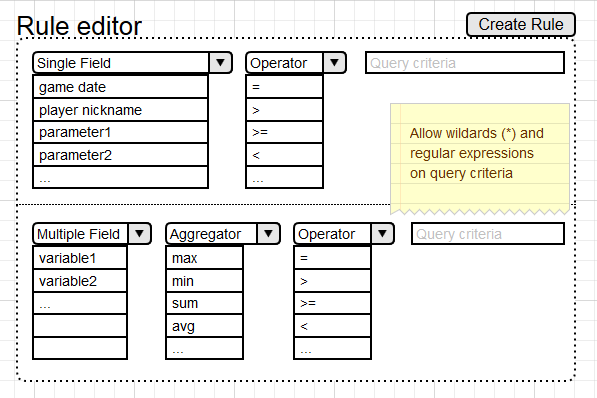
\includegraphics[scale=0.65]{figures/analysis.png}
	\caption{Example UI for a local query criteria rule generator}
	\label{fig:analysis}
\end{figure}

The result of this query, using global and/or local game criteria, might again be a JSON file. An advanced analysis environment might also implement a relational mapping of JSON game data so that the query result can be displayed in tables in an online view or provided as table based csv-export for example for spreadsheet programs. If implemented in a generic way, such a mapping might be the basis of an ORM so that BGE can be used together with relational databases as well.

\subsection{Tabular output}
\label{sub:conclusion:table}

In the current implementation, variable outcomes are visualised with charts, giving all players complete information about that variable. A chart furthermore only visualises one variable at a time. Rendering output as tables might be used to address both issues, enabling incomplete information as well as displaying related things in one place. 

Listing \ref{lst:table} shows how table-based output could be realised in the BGD game code using the example of the order input variable in the beergame which should have incomplete information.

\begin{lstlisting}[language=Javascript, caption=BGD table extension: orders in the beergame, label=lst:table,float,floatplacement=H]
// Custom table showing each player of the beergame only the orders 
// he is allowed to see (incomplete information)
function orderTable(playerIndex) {
    var cr = game.getCurrentRound();
    var table = {};
    table.header = 'Order table in round' + (cr+1);
    table.columns = [];
    // First row of the table. Will be printed in bold by default.
    table.columns.push("Round number", "Orders from client");
    // Go through all rounds and add orders from player's client
    var orders;
    var orderDelay = game.getParameter("orderReceivingDelay");
    for (var roundIndex = 0; roundIndex <= cr; roundIndex++) {
        var orderRoundNumber = roundIndex - orderDelay;
        if (playerIndex === 0) { // retailer
            orders = game.get("customerDemand", orderRoundNumber);
        } else { // wholesaler, distributor, factory
            orders = game.get("order", orderRoundNumber, playerIndex-1);
        }
        table.columns.push(roundIndex + 1, orders);
    }
    return table; // Each custom-defined table must return such an object
}
// Register tables in the architecture
game.registerTables([orderTable, otherCustomTable, preDefinedTable, ...]);

/*
There might be other pre-defined tables such as 
roundResultTable (all players' variable results of the last round)
or playerResultTable (all variable results of this player for all rounds).
These tables could also be registered with the game.registerTables() method.
*/
\end{lstlisting}


%% Optional: Anhang
\appendix
\chapter{Appendix}
\section{Stone-paper-scissors} \label{App:AppendixA}
\begin{lstlisting}[language=Javascript, caption=Game code of stone-paper-scissors, label=lst:sps]
//Schnick Schnack Schnuck
game.addParameter("maxRounds", 10, [
    ">=1",
    "%1===0"
]);
game.addParameter("minPlayers", 2, ["===2"]);
game.addParameter("maxPlayers", 2, ["===2"]);
game.addParameter("roundTimeOut", 20, [
    ">=15",
    "%1===0"
]);
/* Choice-Set. Left term must beat the right term in order to make 
the winner function work. */
var choiceSet = [
        "Stone",
        "Scissors",
        "Paper"
    ];
/*var choiceSet = ["cockroach", "nuclear bomb", "foot"];*/
/*
 Input: Stone, Scissors or Paper
 */
var choice = {
        name: "choice",
        scrollDown: {
            values: choiceSet,
            default: choiceSet[0]
        },
        calculationFunction: bot
    };
game.addInputVariable(choice);
function bot(playerIndex) {
    var result = "Error";
    var randomInt = game.math.randomInt(0, 2);
    result = choiceSet[randomInt];
    return result;
}
/*
 Integer variable. -1 if a player looses the round, 1 if he wins, 0 for tie
 */
var winner = {
        name: "roundWinner",
        type: Number,
        initialValue: [
            0,
            0
        ],
        calculationFunction: calcWinner,
        validation: [
            ">=-1",
            "<=1",
            "%1===0"
        ]
    };
game.addPlayerVariable(winner);
function calcWinner(playerIndex) {
    var result = Number.MIN_VALUE;
    var cr = game.getCurrentRound();
    var player1Choice = choiceToInt(game.get("choice", cr, 0));
    var player2Choice = choiceToInt(game.get("choice", cr, 1));
    var diff;
    if (playerIndex === 0) {
        diff = player1Choice - player2Choice;
    } else {
        diff = player2Choice - player1Choice;
    }
    if (diff === -1 || diff === 2) {
        result = 1;
    } else if (diff === 0) {
        result = 0;
    } else {
        result = -1;
    }
    return result;
}
function choiceToInt(choice) {
    var result = Number.MIN_VALUE;
    for (var i = 0; i < choiceSet.length; i++) {
        if (choice === choiceSet[i]) {
            result = i;
            break;
        }
    }
    return result;
}
/*
 Score Function
 */
function scoreFunction(playerIndex) {
    var result = Number.MIN_VALUE;
    var cr = game.getCurrentRound();
    result = game.get("roundWinner", cr, playerIndex);
    // result = calcWinner(playerIndex);
    return result;
}
var winner = {
        caption: "Game score",
        type: "lineChart",
        unit: "points",
        xInit: game.utils.getWeekNumber(new Date()),
        xIncrement: 1
    };
game.addScore(scoreFunction, winner);
\end{lstlisting}
\section{Beergame} \label{App:beer}
\begin{lstlisting}[language=Javascript, caption=Game code of the beergame, label=lst:beergame]
/* 
Beer distribution game for 4 players with different roles (Retailer,
Wholesaler, Distributor, Factory).
"Role-behaviour" is not yet implemented, maybe in version 2.
Therefore: Player 1 --> Retailer (R), Player 2 --> Wholesaler (W),
Player 3 --> Distributor (D), Player 4 --> Factory (F)
*/
game.addParameter("maxRounds", 30, [
    ">=1",
    "%1===0"
]);
// show more to players to avoid horizon effects
game.addParameter("minPlayers", 4, ["===4"]);
game.addParameter("maxPlayers", 4, ["===4"]);
game.addParameter("roundTimeOut", 90, [
    ">=15",
    "%1===0"
]);
game.addParameter("orderReceivingDelay", 1, [
    ">=0",
    "%1===0"
]);
// 1 round (=1 week)
game.addParameter("shipping/productionDelay", 4, [
    ">=1",
    "%1===0"
]);
// 4 weeks
game.addParameter("inventoryHoldingCosts", 0.5, [">0"]);
// 0.5$ per case per week
game.addParameter("backlogCosts", 1, [">0"]);
// 1$ per case per week
/*
Order (cases/week) input variable
*/
var order = {
        name: "orders",
        initialValue: 4,
        textField: {
            type: "number",
            default: 6,
            validation: [
                ">=0",
                "%1===0"
            ]
        },
        calculationFunction: orderBot
    };
var orderChart = {
        caption: "Beer orders",
        type: "lineChart",
        unit: "cases of beer",
        xInit: game.utils.getWeekNumber(new Date()),
        xIncrement: 1
    };
game.addInputVariable(order, orderChart);
function orderBot(playerIndex) {
    var result = Number.MIN_VALUE;
    // as described in Sterman's Paper: the first four rounds
    // everybody orders 4 cases
    var cr = game.getCurrentRound();
    if (cr < 4) {
        result = 4;
    }    // after 4 rounds the players can order as they want
    else if (cr >= 4) {
        result = game.math.randomInt(6, 20);
    }
    return result;
}
/*
Collective and individual score functions.
Aim of the players: Minimize the total (collective) cost of
the whole beer distributing organisation while only having
local information about the individual costs (the costs for
backlog and inventory in each round).
--> costs = score are a negative number.
*/
function scoreFunction(playerIndex) {
    var result = Number.MAX_VALUE;
    var cr = game.getCurrentRound();
    result = game.get("totalCost", cr, playerIndex);
    return result;
}
var totalCostss = {
        caption: "Total cost",
        type: "columnChart",
        unit: "Euros",
        xInit: game.utils.getWeekNumber(new Date()),
        xIncrement: 1
    };
game.addScore(scoreFunction, totalCostss);
function collectiveScoreFunction() {
    var result = 0;
    var cr = game.getCurrentRound();
    for (var i = 0; i < game.getNumberOfPlayers(); i++) {
        result += Number(game.get("roundScore", cr, i));
    }
    return result;
}
game.addCollectiveScore(collectiveScoreFunction);
/*
Customer demand (cases/week) variable
*/
var customerDemand = {
        name: "customerDemand",
        initialValue: 4,
        calculationFunction: getCustDemand,
        validation: [
            ">=0",
            "%1===0"
        ]
    };
game.addRoundVariable(customerDemand);
function getCustDemand() {
    var result = Number.MIN_VALUE;
    var cr = game.getCurrentRound();
    // "The first four weeks of play are used to familiarize the
    subjects with the mechanics..." of the game
    if (cr >= 0 && cr <= 3) {
        result = 4;
    }    // "There is an unannounced, one-time increase in customer
         // demand to eight cases per week in week 5"
    else if (cr > 3) {
        result = 8;
    }
    return result;
}
/*
Incoming beer cases from the next bigger in the supply chain.
*/
var incomingInventory = {
        name: "incomingInventory",
        initialValue: 4,
        calculationFunction: calcIncoming,
        validation: [
            ">=0",
            "%1===0"
        ]
    };
game.addPlayerVariable(incomingInventory);
function calcIncoming(playerIndex) {
    // playerIndex always starts at 0 (for Player 1)
    var result = Number.MIN_VALUE;
    var cr = game.getCurrentRound();
    var incomingRoundNumber = cr - game.getParameter("shipping/productionDelay");
    // R, W, D incoming inventory is defined by outgoing inventory
    // of the next bigger in the supply chain (after shipping delay)
    if (playerIndex < 3) {
        result = game.get("outgoingInventory", incomingRoundNumber,
        playerIndex + 1);
    }    // Factory (Player 4): Incoming is what Factory ordered to produce 
    else if (playerIndex === 3) {
        result = game.get("orders", incomingRoundNumber, 3);
    }
    return result;
}
/*
Total orders are incoming orders from the next smaller in the 
supply chain plus an eventual backlog from last week.
*/
var totalOrders = {
        name: "totalOrders",
        calculationFunction: calcTotalOrders,
        validation: [
            ">=0",
            "%1===0"
        ]
    };
game.addPlayerVariable(totalOrders);
function calcTotalOrders(playerIndex) {
    var result = Number.MIN_VALUE;
    var cr = game.getCurrentRound();
    var orderRoundNumber = cr - game.getParameter("orderReceivingDelay");
    var ordersFromDownstream = Number.MIN_VALUE;
    // R receives orders from customers    
    if (playerIndex === 0) {
        ordersFromDownstream = game.get("customerDemand", orderRoundNumber);
    }    // W,D,F receive orders from the next smaller in the supply
    chain
    else if (playerIndex > 0) {
        ordersFromDownstream = game.get("orders", orderRoundNumber,
        playerIndex - 1);
    }
    // Total orders are the incoming orders + an eventual backlog
    // from last week
    var backlogLastWeek = Number.MIN_VALUE;
    var inventoryLastWeek = game.get("inventory", cr - 1, playerIndex);
    if (inventoryLastWeek < 0) {
        backlogLastWeek = -1 * inventoryLastWeek;
    } else if (inventoryLastWeek >= 0) {
        backlogLastWeek = 0;
    }
    result = backlogLastWeek + ordersFromDownstream;
    return result;
}
/*
Outgoing beer cases which are shipped to the next smaller in the
supply chain.
*/
var outgoingInventory = {
        name: "outgoingInventory",
        initialValue: 4,
        calculationFunction: calcOutgoing,
        validation: [
            ">=0",
            "%1===0"
        ]
    };
game.addPlayerVariable(outgoingInventory);
function calcOutgoing(playerIndex) {
    var result = Number.MIN_VALUE;
    var cr = game.getCurrentRound();
    var incoming = game.get("incomingInventory", cr, playerIndex);
    var inventoryLastWeek = game.get("inventory", cr - 1, playerIndex);
    var totalOrders = game.get("totalOrders", cr, playerIndex);
    // calculate number of outgoing beer cases. 
    if (inventoryLastWeek < 0) {
        result = Math.min(incoming, totalOrders);
    } else if (inventoryLastWeek >= 0) {
        result = Math.min(inventoryLastWeek + incoming, totalOrders);
    }
    return result;
}
/*
A negative inventory means backlog.
*/
var inventory = {
        name: "inventory",
        initialValue: 12,
        calculationFunction: calcInventory,
        validation: ["%1===0"]
    };
var inventChart = {
        caption: "Inventory",
        type: "columnChart",
        unit: "Cases of beer",
        xInit: game.utils.getWeekNumber(new Date()),
        xIncrement: 1
    };
game.addPlayerVariable(inventory, inventChart);
function calcInventory(playerIndex) {
    var result = -0.5;
    var cr = game.getCurrentRound();
    var totalOrders = game.get("totalOrders", cr, playerIndex);
    var incoming = game.get("incomingInventory", cr, playerIndex);
    var inventoryLastWeek = game.get("inventory", cr - 1, playerIndex);
    if (inventoryLastWeek < 0) {
        result = incoming - totalOrders; // backlog of last week
                                         // is already in the total orders
    } else if (inventoryLastWeek >= 0) {
        result = inventoryLastWeek + incoming - totalOrders;
    }
    return result;
}
/*
Backlog costs.
Costs are a negative number. --> the bigger the number, the better.
*/
var backlogCost = {
        name: "backlogCost",
        initialValue: 0,
        calculationFunction: calcBacklogCost,
        validation: ["<=0"]
    };
var backlogChart = {
        caption: "Backlog costs",
        type: "columnChart",
        unit: "Euros",
        xInit: game.utils.getWeekNumber(new Date()),
        xIncrement: 1
    };
game.addPlayerVariable(backlogCost, backlogChart);
function calcBacklogCost(playerIndex) {
    var result = 0;
    var cr = game.getCurrentRound();
    var inventory = game.get("inventory", cr, playerIndex);
    if (inventory < 0) {
        result = game.getParameter("backlogCosts") * inventory;
    }
    return result;
}
/*
Inventory holding costs.
Costs are a negative number.
*/
var invHolding = {
        name: "inventoryHoldingCost",
        initialValue: 0,
        calculationFunction: calcInvHolding,
        validation: ["<=0"]
    };
var invHoldingChart = {
        caption: "Inventory holding costs",
        type: "columnChart",
        unit: "Euros",
        xInit: game.utils.getWeekNumber(new Date()),
        xIncrement: 1
    };
game.addPlayerVariable(invHolding, invHoldingChart);
function calcInvHolding(playerIndex) {
    var result = 0;
    var cr = game.getCurrentRound();
    var inventory = game.get("inventory", cr, playerIndex);
    if (inventory > 0) {
        result = game.getParameter("inventoryHoldingCosts") * -1 * inventory;
    }
    return result;
}
/*
Total costs = backlog costs + inventory holding costs
Costs are a negative number.
*/
var totalCost = {
        name: "totalCost",
        initialValue: 0,
        calculationFunction: calcTotalCost,
        validation: ["<=0"]
    };
game.addPlayerVariable(totalCost);
function calcTotalCost(playerIndex) {
    var result = Number.MAX_VALUE;
    var cr = game.getCurrentRound();
    var bc = game.get("backlogCost", cr, playerIndex);
    var ihc = game.get("inventoryHoldingCost", cr, playerIndex);
    result = bc + ihc;
    return result;
}
\end{lstlisting}

\cleardoublepage

%% Literatur
\addcontentsline{toc}{chapter}{\bibname}


\IfLanguageName{ngerman}{
\bibliographystyle{em_includes/emalphde}
% Alphanumerische Zitierung (EM Style), deutsch. Ggf. durch andere Varianten 
% im Ordner em_includes austauschen.
}{
\bibliographystyle{em_includes/emalphen}
% Alphanumeric Citation (EM Style), English.
}

\nocite{*} % Alle Quellen anzeigen, die im Bibfile stehen, auch wenn sie nicht im Text referenziert wurden
\bibliography{literature}

%% Index
%\addcontentsline{toc}{chapter}{\indexname}
\printindex            % Index, Stichwortverzeichnis

\end{document}
%% end of file
